% Options for packages loaded elsewhere
\PassOptionsToPackage{unicode}{hyperref}
\PassOptionsToPackage{hyphens}{url}
%
\documentclass[
]{article}
\usepackage{lmodern}
\usepackage{amssymb,amsmath}
\usepackage{ifxetex,ifluatex}
\ifnum 0\ifxetex 1\fi\ifluatex 1\fi=0 % if pdftex
  \usepackage[T1]{fontenc}
  \usepackage[utf8]{inputenc}
  \usepackage{textcomp} % provide euro and other symbols
\else % if luatex or xetex
  \usepackage{unicode-math}
  \defaultfontfeatures{Scale=MatchLowercase}
  \defaultfontfeatures[\rmfamily]{Ligatures=TeX,Scale=1}
\fi
% Use upquote if available, for straight quotes in verbatim environments
\IfFileExists{upquote.sty}{\usepackage{upquote}}{}
\IfFileExists{microtype.sty}{% use microtype if available
  \usepackage[]{microtype}
  \UseMicrotypeSet[protrusion]{basicmath} % disable protrusion for tt fonts
}{}
\makeatletter
\@ifundefined{KOMAClassName}{% if non-KOMA class
  \IfFileExists{parskip.sty}{%
    \usepackage{parskip}
  }{% else
    \setlength{\parindent}{0pt}
    \setlength{\parskip}{6pt plus 2pt minus 1pt}}
}{% if KOMA class
  \KOMAoptions{parskip=half}}
\makeatother
\usepackage{xcolor}
\IfFileExists{xurl.sty}{\usepackage{xurl}}{} % add URL line breaks if available
\IfFileExists{bookmark.sty}{\usepackage{bookmark}}{\usepackage{hyperref}}
\hypersetup{
  pdftitle={Police Shootings and Racism in America},
  pdfauthor={Connie Wu},
  hidelinks,
  pdfcreator={LaTeX via pandoc}}
\urlstyle{same} % disable monospaced font for URLs
\usepackage[margin=1in]{geometry}
\usepackage{graphicx,grffile}
\makeatletter
\def\maxwidth{\ifdim\Gin@nat@width>\linewidth\linewidth\else\Gin@nat@width\fi}
\def\maxheight{\ifdim\Gin@nat@height>\textheight\textheight\else\Gin@nat@height\fi}
\makeatother
% Scale images if necessary, so that they will not overflow the page
% margins by default, and it is still possible to overwrite the defaults
% using explicit options in \includegraphics[width, height, ...]{}
\setkeys{Gin}{width=\maxwidth,height=\maxheight,keepaspectratio}
% Set default figure placement to htbp
\makeatletter
\def\fps@figure{htbp}
\makeatother
\setlength{\emergencystretch}{3em} % prevent overfull lines
\providecommand{\tightlist}{%
  \setlength{\itemsep}{0pt}\setlength{\parskip}{0pt}}
\setcounter{secnumdepth}{-\maxdimen} % remove section numbering

\title{Police Shootings and Racism in America}
\author{Connie Wu}
\date{10/17/2020}

\begin{document}
\maketitle

\hypertarget{i.-introduction}{%
\subsection{I. Introduction}\label{i.-introduction}}

~~~~~~~On May 25, 2020, George Floyd was publicly suffocated to death by
police officers in Minneapolis, Minnesota. This, along with the murder
of Breonna Taylor by Louisville police, incited waves of protests
against police brutality across the United States and increased the
spread of Black Lives Matter content on social media. The recent boost
in attention to the Black Lives Matter movement has once again brought
to light the issue of racism in America and its link to police
brutality, and more specifically, police use of deadly force. Several
studies have already found that race does play a part in who is targeted
and killed in police shootings. For example, in a recent VICE News
investigation about police shootings, it was found that ``Black people
were shot more often and at higher rates than people of any other
race.'' {[}1{]} Additionally, Edwards et. al performed a study regarding
the effects of age, race-ethnicity, and sex on the risk of being killed
by lethal force by law enforcement and similarly found that ``Black men
are about 2.5 times more likely to be killed by police over the life
course than are white men'' while ``Black women are about 1.4 times more
likely to be killed by police than are white women.'' {[}2{]} However,
even with these studies and their disturbing conclusions, a poll done by
AP-NORC in June 2020 found that still 39\% of Americans think that
police are not more likely to use lethal force against a Black person
than a White person. {[}3{]} Although this has decreased from an
overwhelming 51\% in June 2015, there is still a great deal of research
that needs to be done in this area to provide more statistical evidence
backing the relationship between racism and police use of deadly
force.\\
\hspace*{0.333em}\hspace*{0.333em}\hspace*{0.333em}\hspace*{0.333em}\hspace*{0.333em}\hspace*{0.333em}\hspace*{0.333em}As
a result, I have decided to build off of VICE News' study and
investigate data on police shootings further to understand the roles
that the race of both victim and officer, as well as other factors such
as their genders, whether they are carrying a weapon, and the total
number of victims in the crime, play in fatal versus non-fatal police
shootings. Additionally, to account for the varying locations of the
homicides, I will be using a dataset found on Kaggle detailing the gun
provisions that are upheld by each state see how gun legislation affects
lethal vs.~non-lethal shootings. I will also add a predictor indicating
whether the state in which the homicide occurred requires de-escalation
training for police officers. Finally, I will explore how the race
demographics of each location relates to police use of deadly force.
This will allow me to better understand how racism has manifested itself
in America's police system and determine whether current attempts to
prevent police use of lethal force are effective or not.

\hypertarget{data}{%
\subsubsection{Data}\label{data}}

~~~~~~~As a basis for this study, I will be using the same dataset that
VICE News used. This dataset contains data on officer-involved shootings
from 47 of the largest local police departments in America, and more
specifically, ``information on 4,117 incidents and 4,400 subjects
{[}(victims){]} over seven years.'' {[}1{]} VICE News provides 34
variables in the dataset, including dates ranging from January 2010 to
September 2016, city, subject race, subject gender, office race, officer
gender, the type of weapon the subject was carrying, and whether the
shooting was fatal or not. Race was broken up into 5 categories: White
(non-Hispanic) (represented as W), Black (non-Hispanic) (B), Asian (A),
Latino (L), Other (O), and Unknown (U). Gender was broken up into 3
categories: Male (M), Female (F), and Unknown (U). Weapon type was
broken up into 6 values: ``gun'', ``knife'', ``replica'', ``other'',
``unknown'', and ``other''. Additionally, there were cases in which
multiple victims and/or multiple officers were present in the shooting.
Each of these scenarios was still represented within one row of the
dataset, but semi-colons were present in the respective victim and
officer columns, separating each individual's information from each
other.\\
\hspace*{0.333em}\hspace*{0.333em}\hspace*{0.333em}\hspace*{0.333em}\hspace*{0.333em}\hspace*{0.333em}Additionally,
to assess the effect of different types of legislation on fatal
vs.~non-fatal police shootings in various states, I will be using a
dataset from Kaggle containing 135 variables that detail whether a
certain gun provision is absent or present in a certain year and U.S.
state for 133 different gun provisions. The years range from 1991 to
2017, and the gun provisions address 14 categories, some of which are
dealer regulations, buyer regulations, prohibitions for high-risk gun
possession, background checks, ammunition regulations, possession
regulations, concealed carry permitting, assault weapons and
large-capacity magazines, child access prevention, gun trafficking, and
domestic violence. A 1 in the gun provision column represents a presence
of the law, and a 0 indicates an absence. I will also add a column to
this gun provision dataset indicating whether a state requires
de-escalation training based off of information reported by APM Report
in 2017, with a 1 meaning the state does require training and a 0
meaning the state does not. There were 16 states that required
de-escalation training as of November 2017. {[}4{]}\\
\hspace*{0.333em}\hspace*{0.333em}\hspace*{0.333em}\hspace*{0.333em}\hspace*{0.333em}\hspace*{0.333em}Finally,
to examine city demographics as a predictor, I will be using population
data from the 2013 American Community Survey that VICE News had already
cleaned and standardized to the shootings dataset, meaning the city
names can be matched up between the two datasets. VICE News most likely
provided only 2013 census data because it is the average year of all the
years represented in the shootings dataset. Furthermore, using census
data only from 2013 requires that we analyze this data under the
assumption that there is no drastic difference in population
demographics between 2010 and 2016. The census data includes 7
variables: the police department and the city it's located in, as well
as the city's Black, Asian, Hispanic, White, and overall total
population in 2013.

\hypertarget{ii.-methods}{%
\subsection{II. Methods}\label{ii.-methods}}

\hypertarget{data-processing}{%
\subsubsection{Data Processing}\label{data-processing}}

~~~~~~~Although the VICE News dataset was already relatively clean with
regards to the victim's data, there was still quite a bit of cleaning
that needed to be done for the race and gender data of the officers. To
clean these columns, I replaced all values that were not ``W'', ``B'',
``A'', ``O'', or ``U'' in the race column with the most informed guess
that I could make about what the values represented. For example,
``A/PI'' values were taken to represent Asian/Pacific Islander and thus
were replaced with ``A'', and ``A/W'' or other values with a ``/'' in
them were typically taken to represent multi-racial individuals and as a
result were replaced with ``O.'' Similar procedures were carried out in
the gender column for officers for values that were not ``M'', ``F'', or
``U''.\\
\hspace*{0.333em}\hspace*{0.333em}\hspace*{0.333em}\hspace*{0.333em}\hspace*{0.333em}\hspace*{0.333em}\hspace*{0.333em}After
this initial cleaning, I created new columns in the same dataset that
represented whether any victims of race Black, White, Asian, or Other
were present in the crime, respectively, and if any male or female
victims were present in the crime, respectively. I also added new
columns to represent the same information for officers (for each race
and gender, whether each was present), and a new column to represent
whether any victim involved in the shooting was shot fatally.
Additionally, I made sure that each weapon type had its own column. All
of these added columns had values of either 0 or 1, with 0 representing
an absence of the variable and 1 a presence. Finally, I filtered out
2,079 rows that had only unknown and NA values for the fatality of the
shooting or the races or genders of the victims or officers, as these
rows did not provide sufficient information for my analysis, and I
selected only the columns I needed, such as whether any victim of the
shooting was shot fatally or not, the genders and races of the victims
and officers, and the weapons that the victims were carrying, if any.\\
\hspace*{0.333em}\hspace*{0.333em}\hspace*{0.333em}\hspace*{0.333em}\hspace*{0.333em}\hspace*{0.333em}\hspace*{0.333em}For
the gun provisions dataset, I created a new column that sums up the
total number of laws listed in the dataset that each state had in 2013
(for the same reason that VICE News used 2013). Additionally, as I
mentioned earlier, I appended a column to this dataset representing
whether a state requires de-escalation training for police officers as
of November 2017. 2017 was used under the assumption that no major event
occurred between September 2016 and November 2017 that caused a sudden
increase in the number of states that require de-escalation training for
police officers. Finally, for the census data, the only cleaning that
needed to be done was extracting the state that each city was in from
the department column so that the census could be easily joined with the
cleaned shootings dataset by city name, as well as the gun provisions
dataset by abbreviated state name.\\
\hspace*{0.333em}\hspace*{0.333em}\hspace*{0.333em}\hspace*{0.333em}\hspace*{0.333em}\hspace*{0.333em}\hspace*{0.333em}After
merging the three datasets, the final dataset consists of 2,031
observations.

\hypertarget{exploratory-data-analysis}{%
\subsubsection{Exploratory Data
Analysis}\label{exploratory-data-analysis}}

\begin{figure}
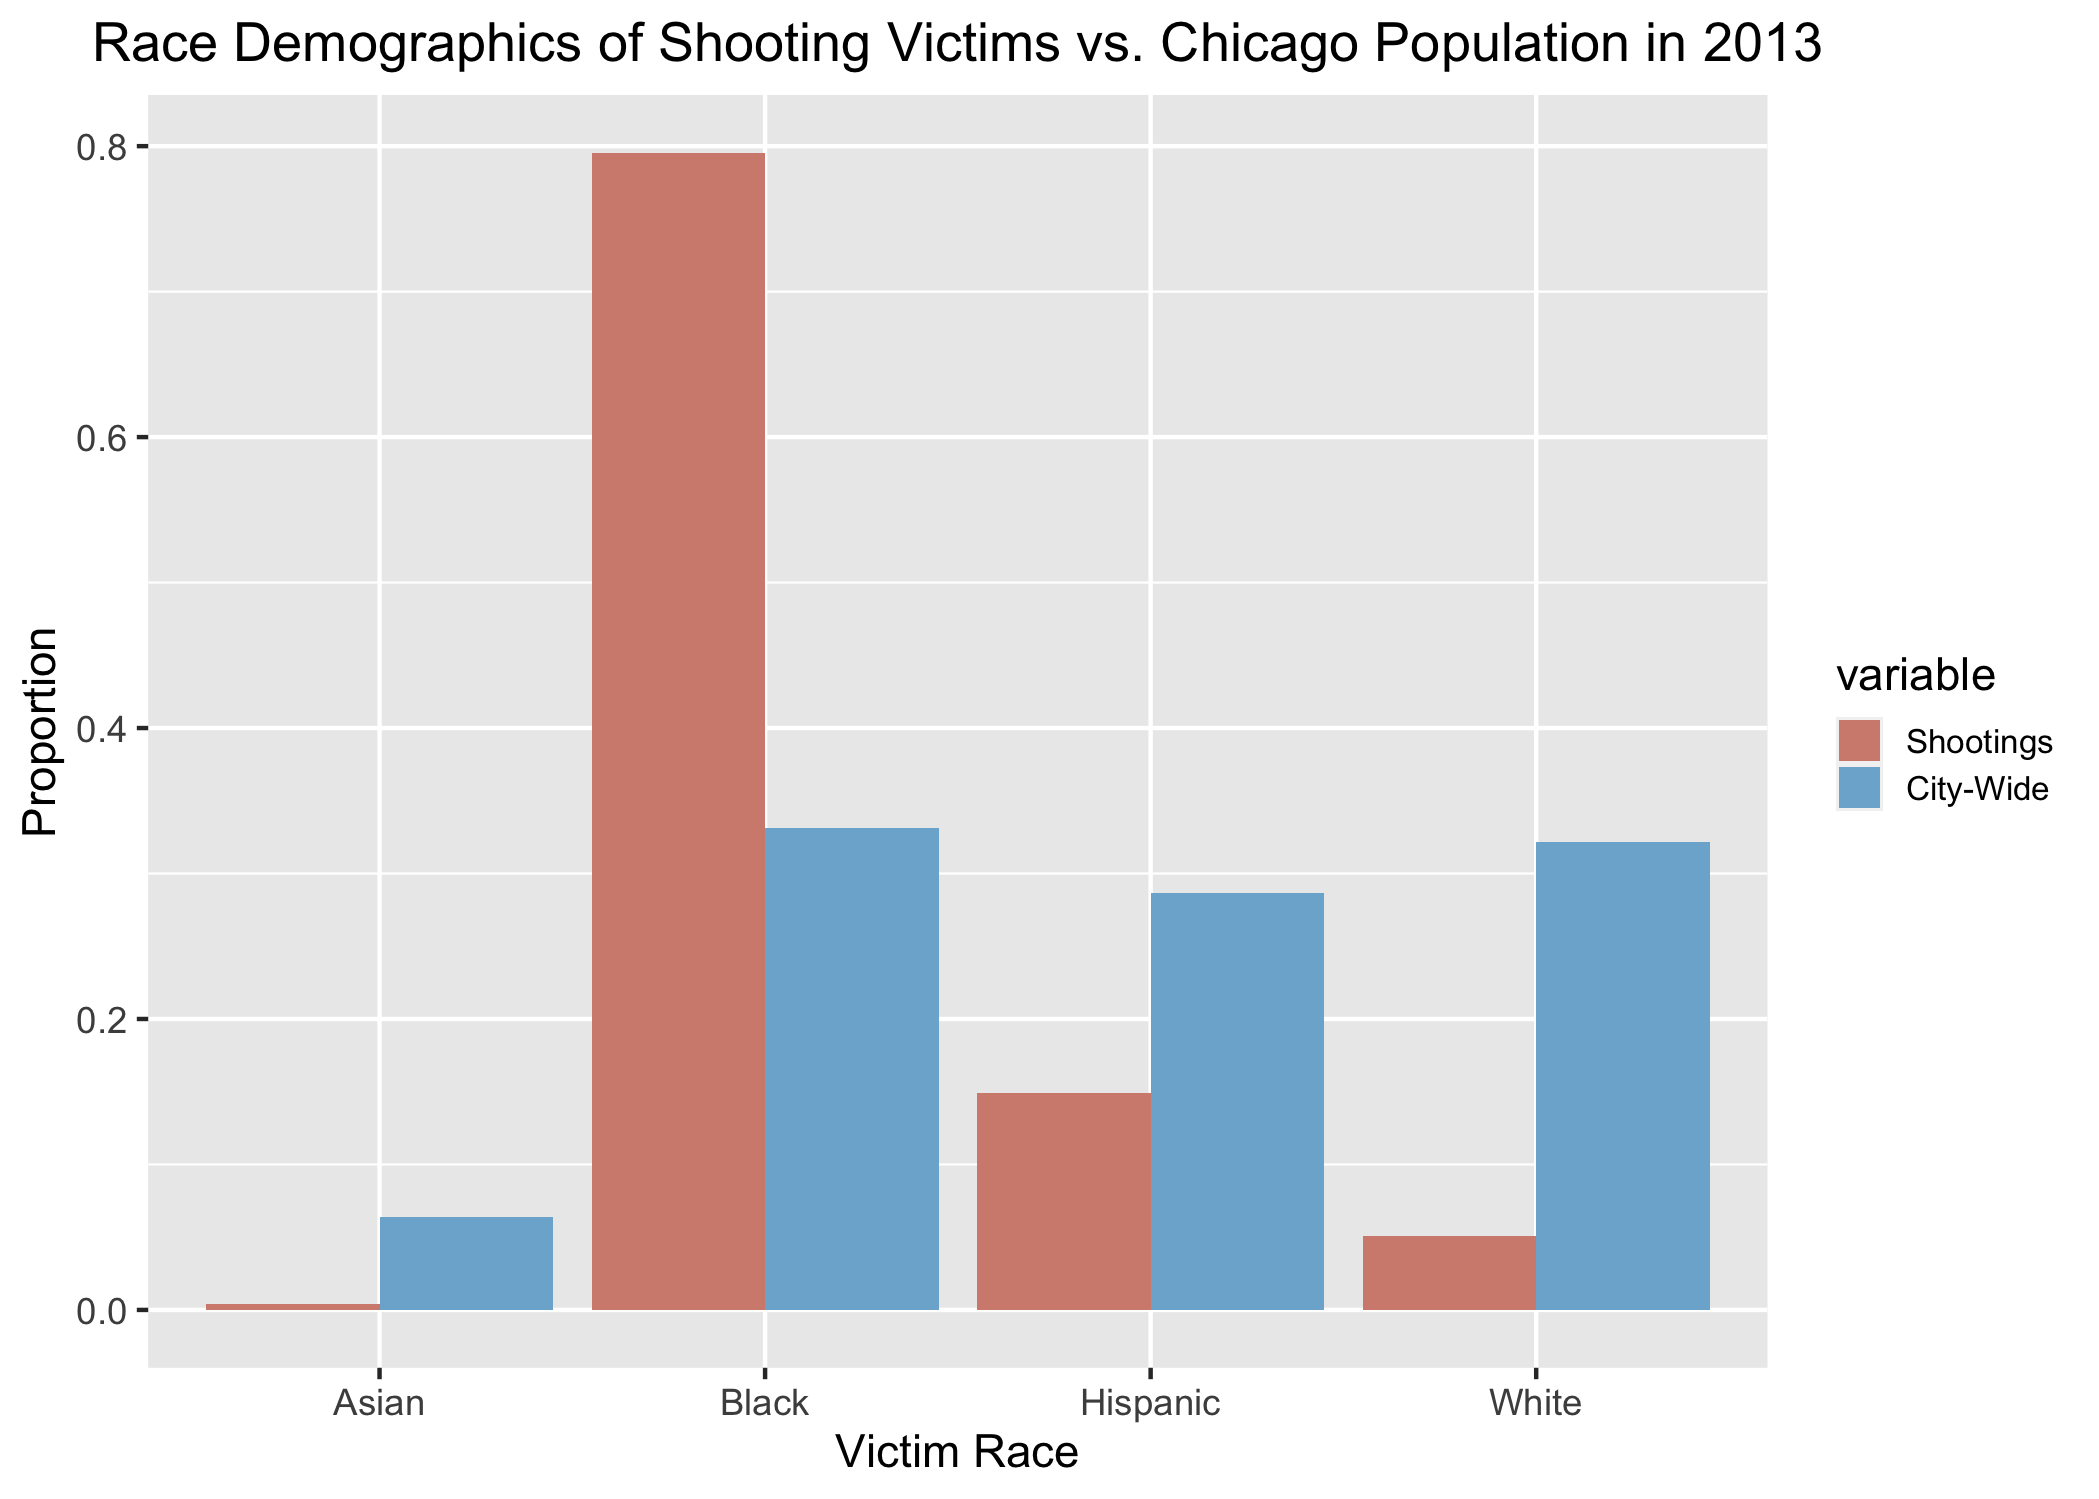
\includegraphics[width=0.25\linewidth]{figures/cityeda1} 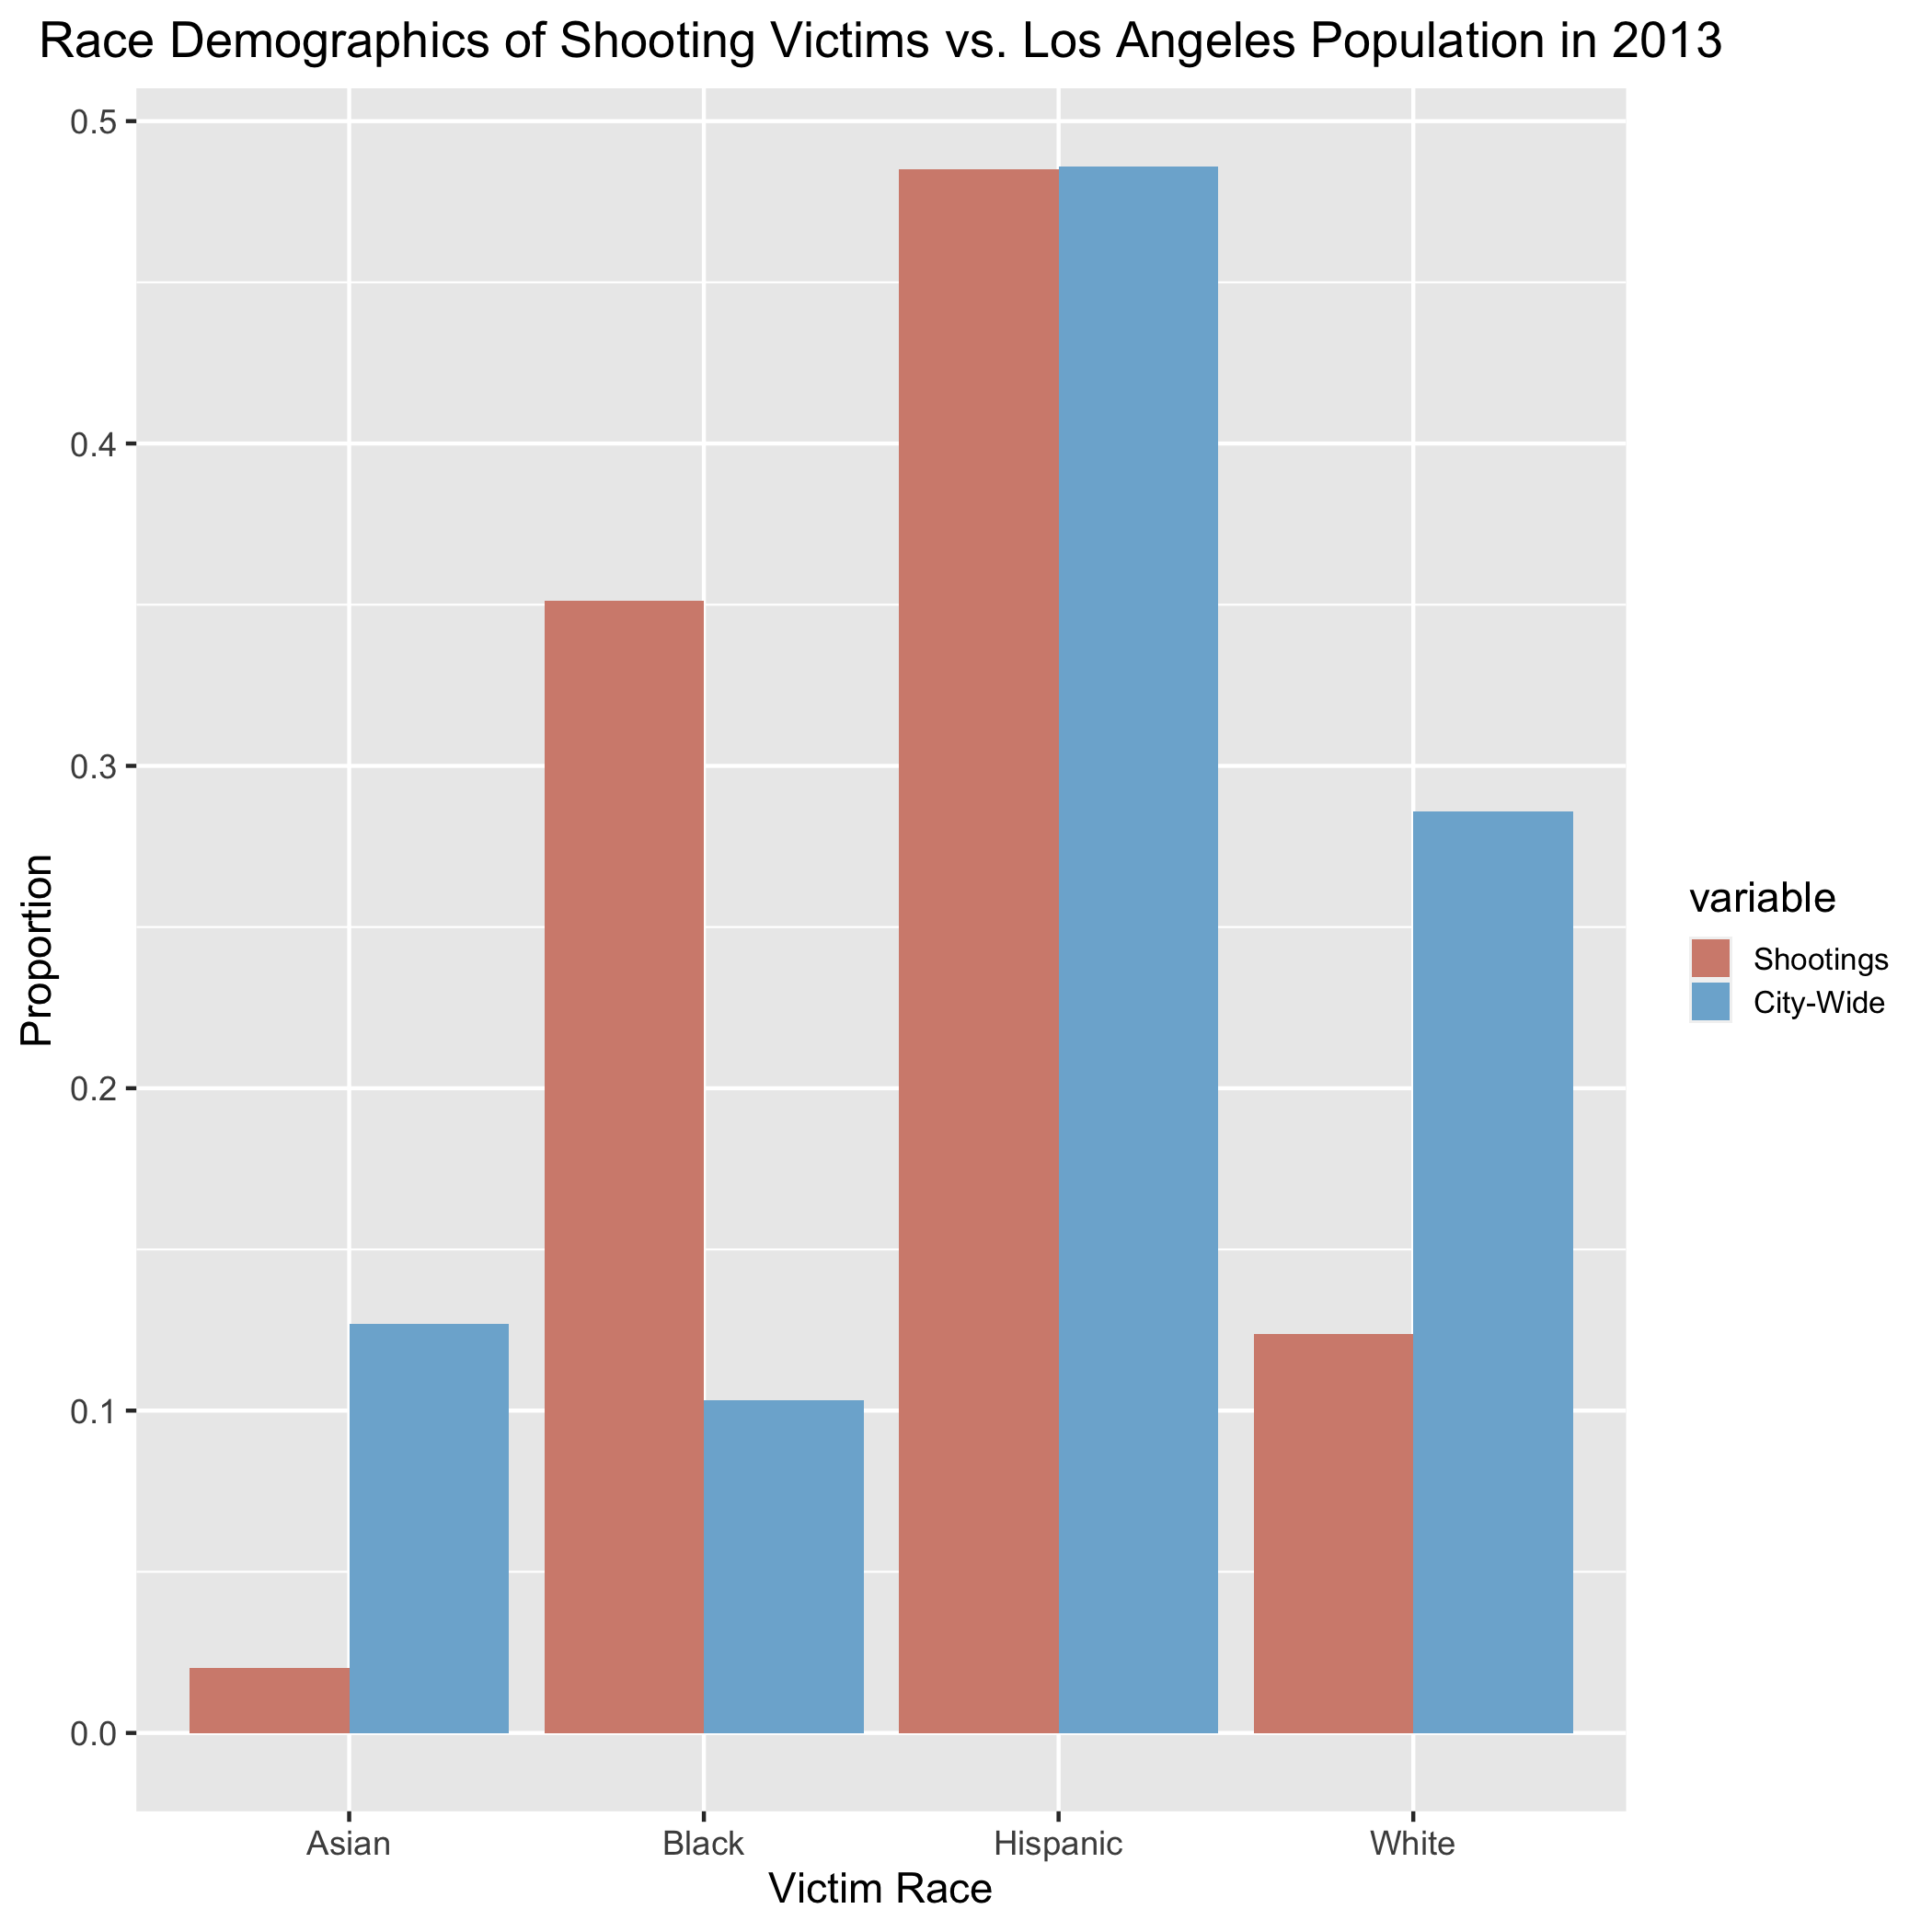
\includegraphics[width=0.25\linewidth]{figures/cityeda2} 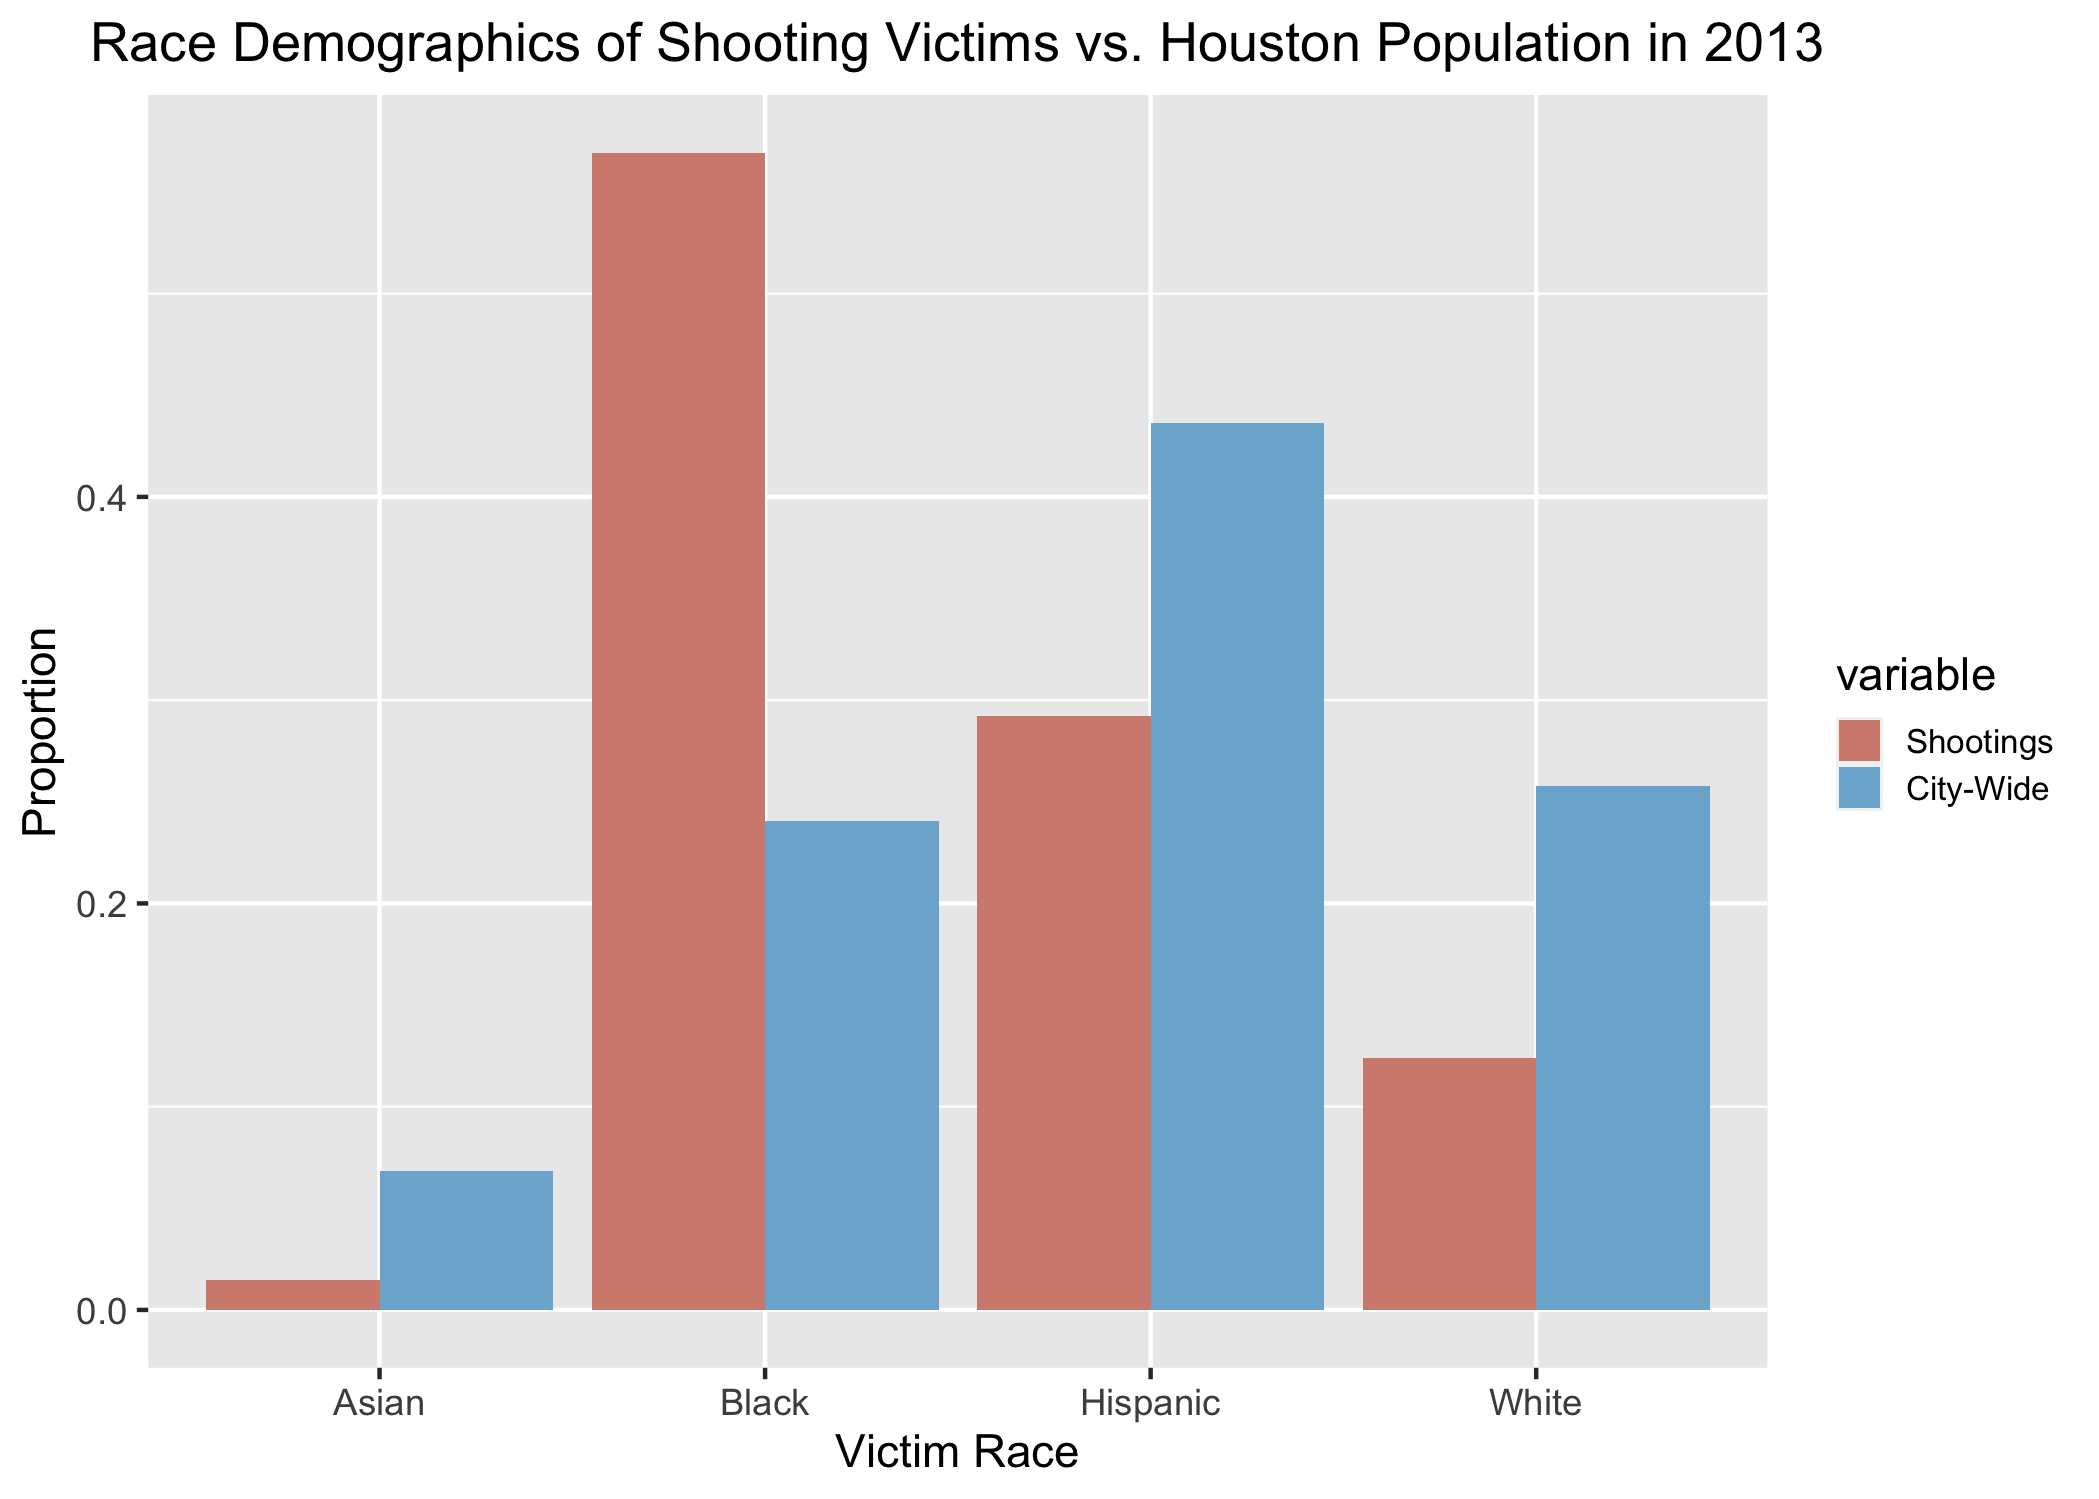
\includegraphics[width=0.25\linewidth]{figures/cityeda3} 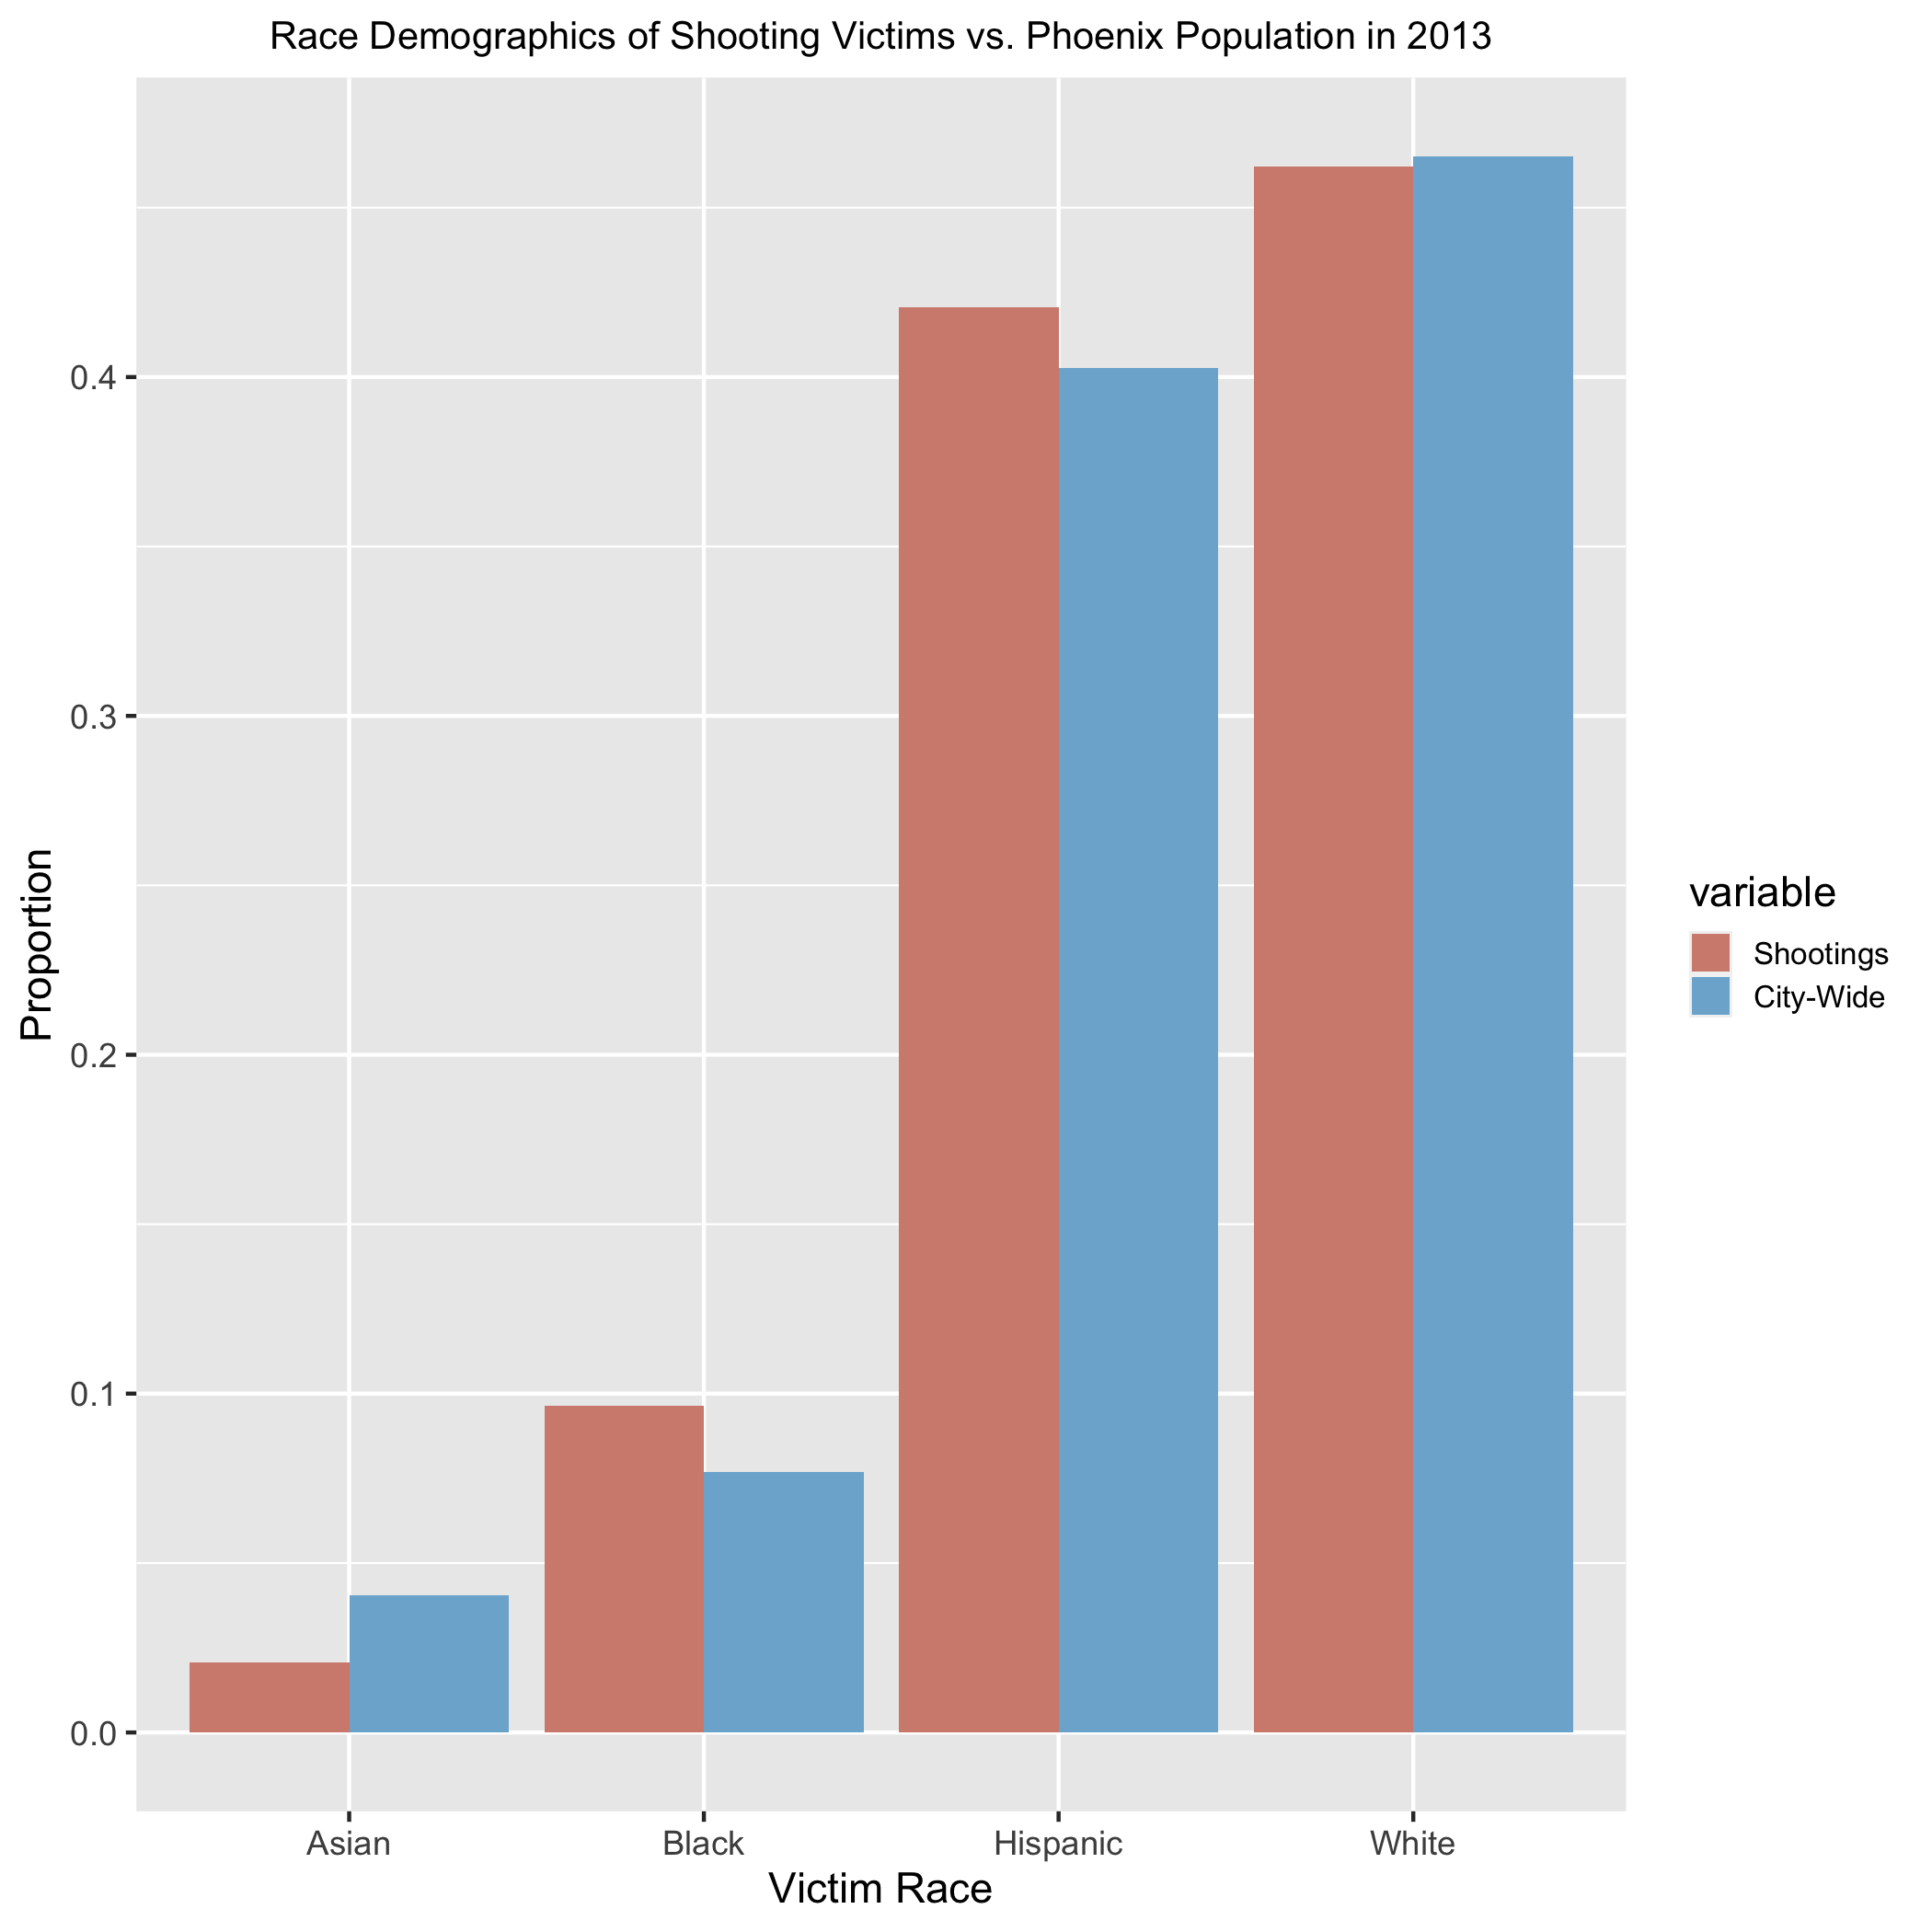
\includegraphics[width=0.25\linewidth]{figures/cityeda4} \caption{Race Proportions of Shooting Victims vs. City Population Demographics of the Most Popular 4 Cities in the Data }\label{fig:figures-city}
\end{figure}

~~~~~~Plotted above in \emph{Figure 1} are the race proportions of
shooting victims in the top 4 most popular cities in the dataset
(Chicago, Los Angeles, Houston, and Phoenix) vs.~the race proportions of
those cities' total populations in 2013. Because the bars representing
shootings in the Black race category are taller than the bars
representing city-wide population in all 4 plots, it is evident Black
people are disproportionately the victims of police shootings compared
to city race proportions. This can especially be seen in Houston, where
Black people make up less than 25\% of the city population yet more than
50\% of the victim population of police shootings.

\begin{figure}
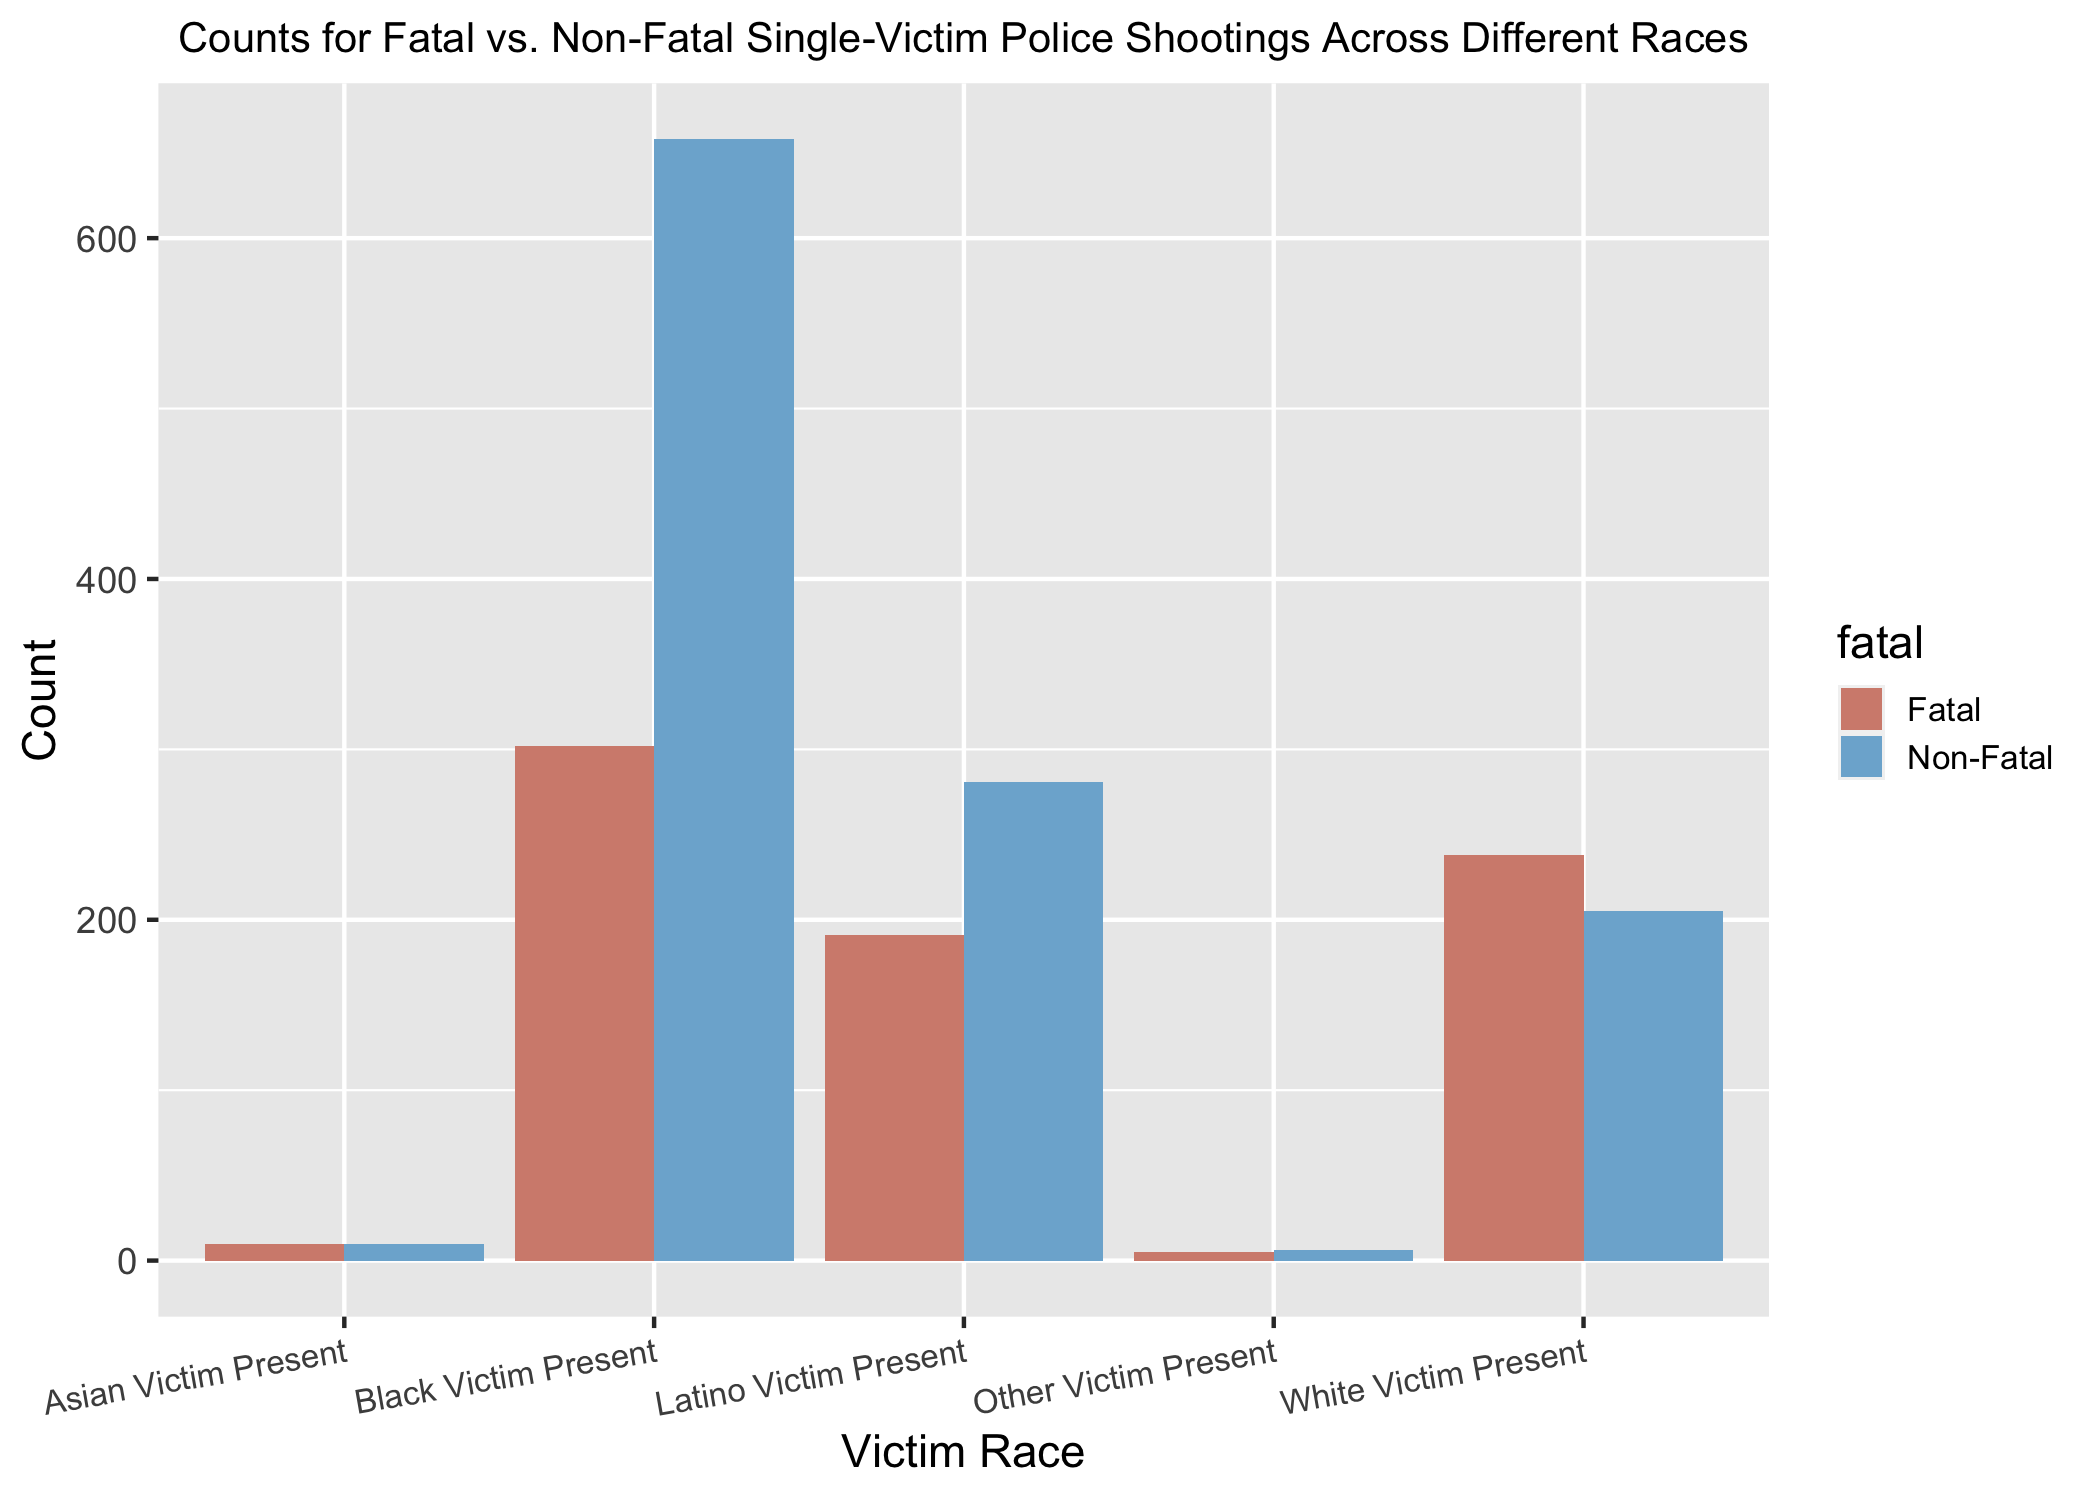
\includegraphics[width=0.5\linewidth]{figures/singleeda1} 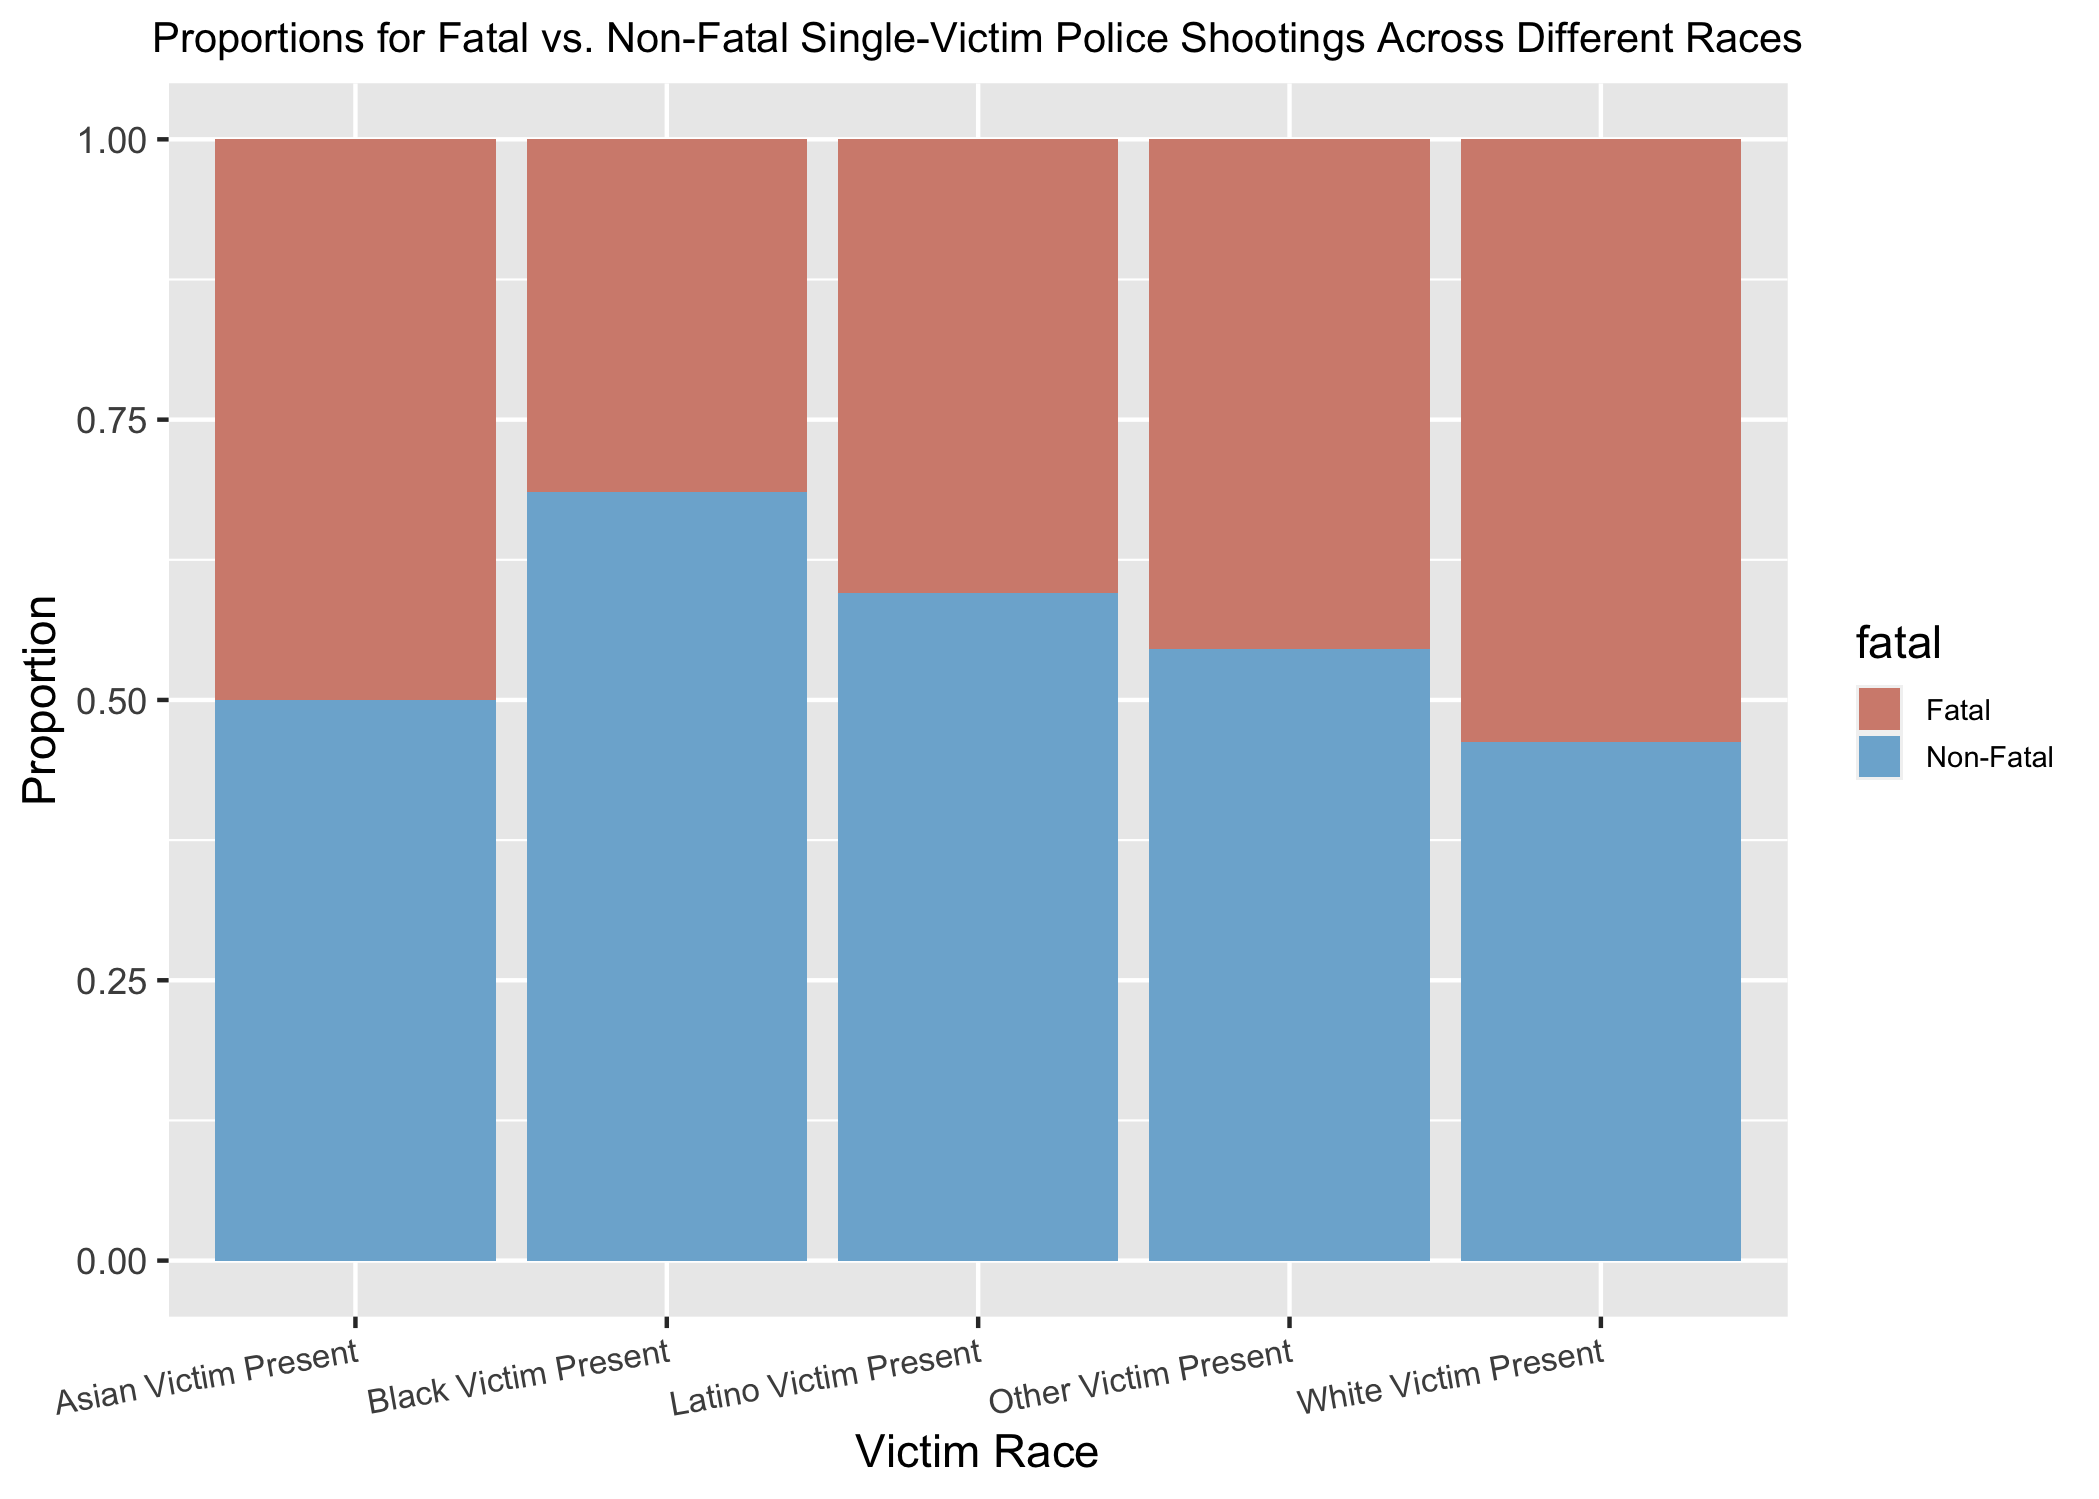
\includegraphics[width=0.5\linewidth]{figures/singleeda2} \caption{Counts (left) and Proportions (right) of Different Races Across Single Victim Shootings}\label{fig:figures-single}
\end{figure}

~~~~~~Additionally, there appears to be 1,906 incidents in the final
dataset in which there was only one victim, and 148 with multiple
victims. Among all shootings with only one victim, it appears in
\emph{Figure 2} that the victim is more often Black than some other
race. However, it seems that Black victims and most victims of the other
race types are more likely to be shot non-fatally than fatally, whereas
White victims seem more likely to be shot fatally. Finally, it is
important to note that the numbers of victims that are of race types
Asian and Other are relatively small. This means that we should proceed
with caution when evaluating the effects of each of these races on
whether a shooting is fatal or non-fatal.\\
\hspace*{0.333em}\hspace*{0.333em}\hspace*{0.333em}\hspace*{0.333em}\hspace*{0.333em}\hspace*{0.333em}Similarly,
Black victims make up the highest proportion of victims in shootings
with multiple victims. However, in these shootings, all race types are
more likely to be shot non-fatally than fatally, with Latinos having the
highest proportion of being shot fatally out of all other race types.
Additionally, it should be noted that there are no victims with race
type ``Other'' in shootings where there are multiple victims. These
graphs can be found as \emph{Figure 3} in the Appendix.

\hypertarget{model}{%
\subsubsection{Model}\label{model}}

~~~~~~~The predictors that I will use are subject race, subject gender,
officer race, officer gender, and the type of weapon the subject was
carrying. The response I will be modeling will be whether the shooting
was fatal or not.

\hypertarget{iii.-preliminary-results}{%
\subsection{III. Preliminary Results}\label{iii.-preliminary-results}}

\begin{itemize}
\tightlist
\item
  limitations: time series, also counting N;U\ldots{} combos as N even
  though some are unknown
\end{itemize}

\hypertarget{references}{%
\subsection{References}\label{references}}

\begin{enumerate}
\def\labelenumi{\arabic{enumi})}
\tightlist
\item
  Vice
\item
  \url{https://www.pnas.org/content/pnas/116/34/16793.full.pdf}
\item
  \url{https://www.kpbs.org/news/2020/jun/18/sweeping-change-us-views-police-violence-new-poll-/}
\item
  \url{http://govred.com/blog/deescalation-training-state-requirements/}
\end{enumerate}

\hypertarget{appendix}{%
\subsection{Appendix}\label{appendix}}

\hypertarget{exploratory-data-analysis-1}{%
\subsubsection{Exploratory Data
Analysis}\label{exploratory-data-analysis-1}}

\begin{figure}
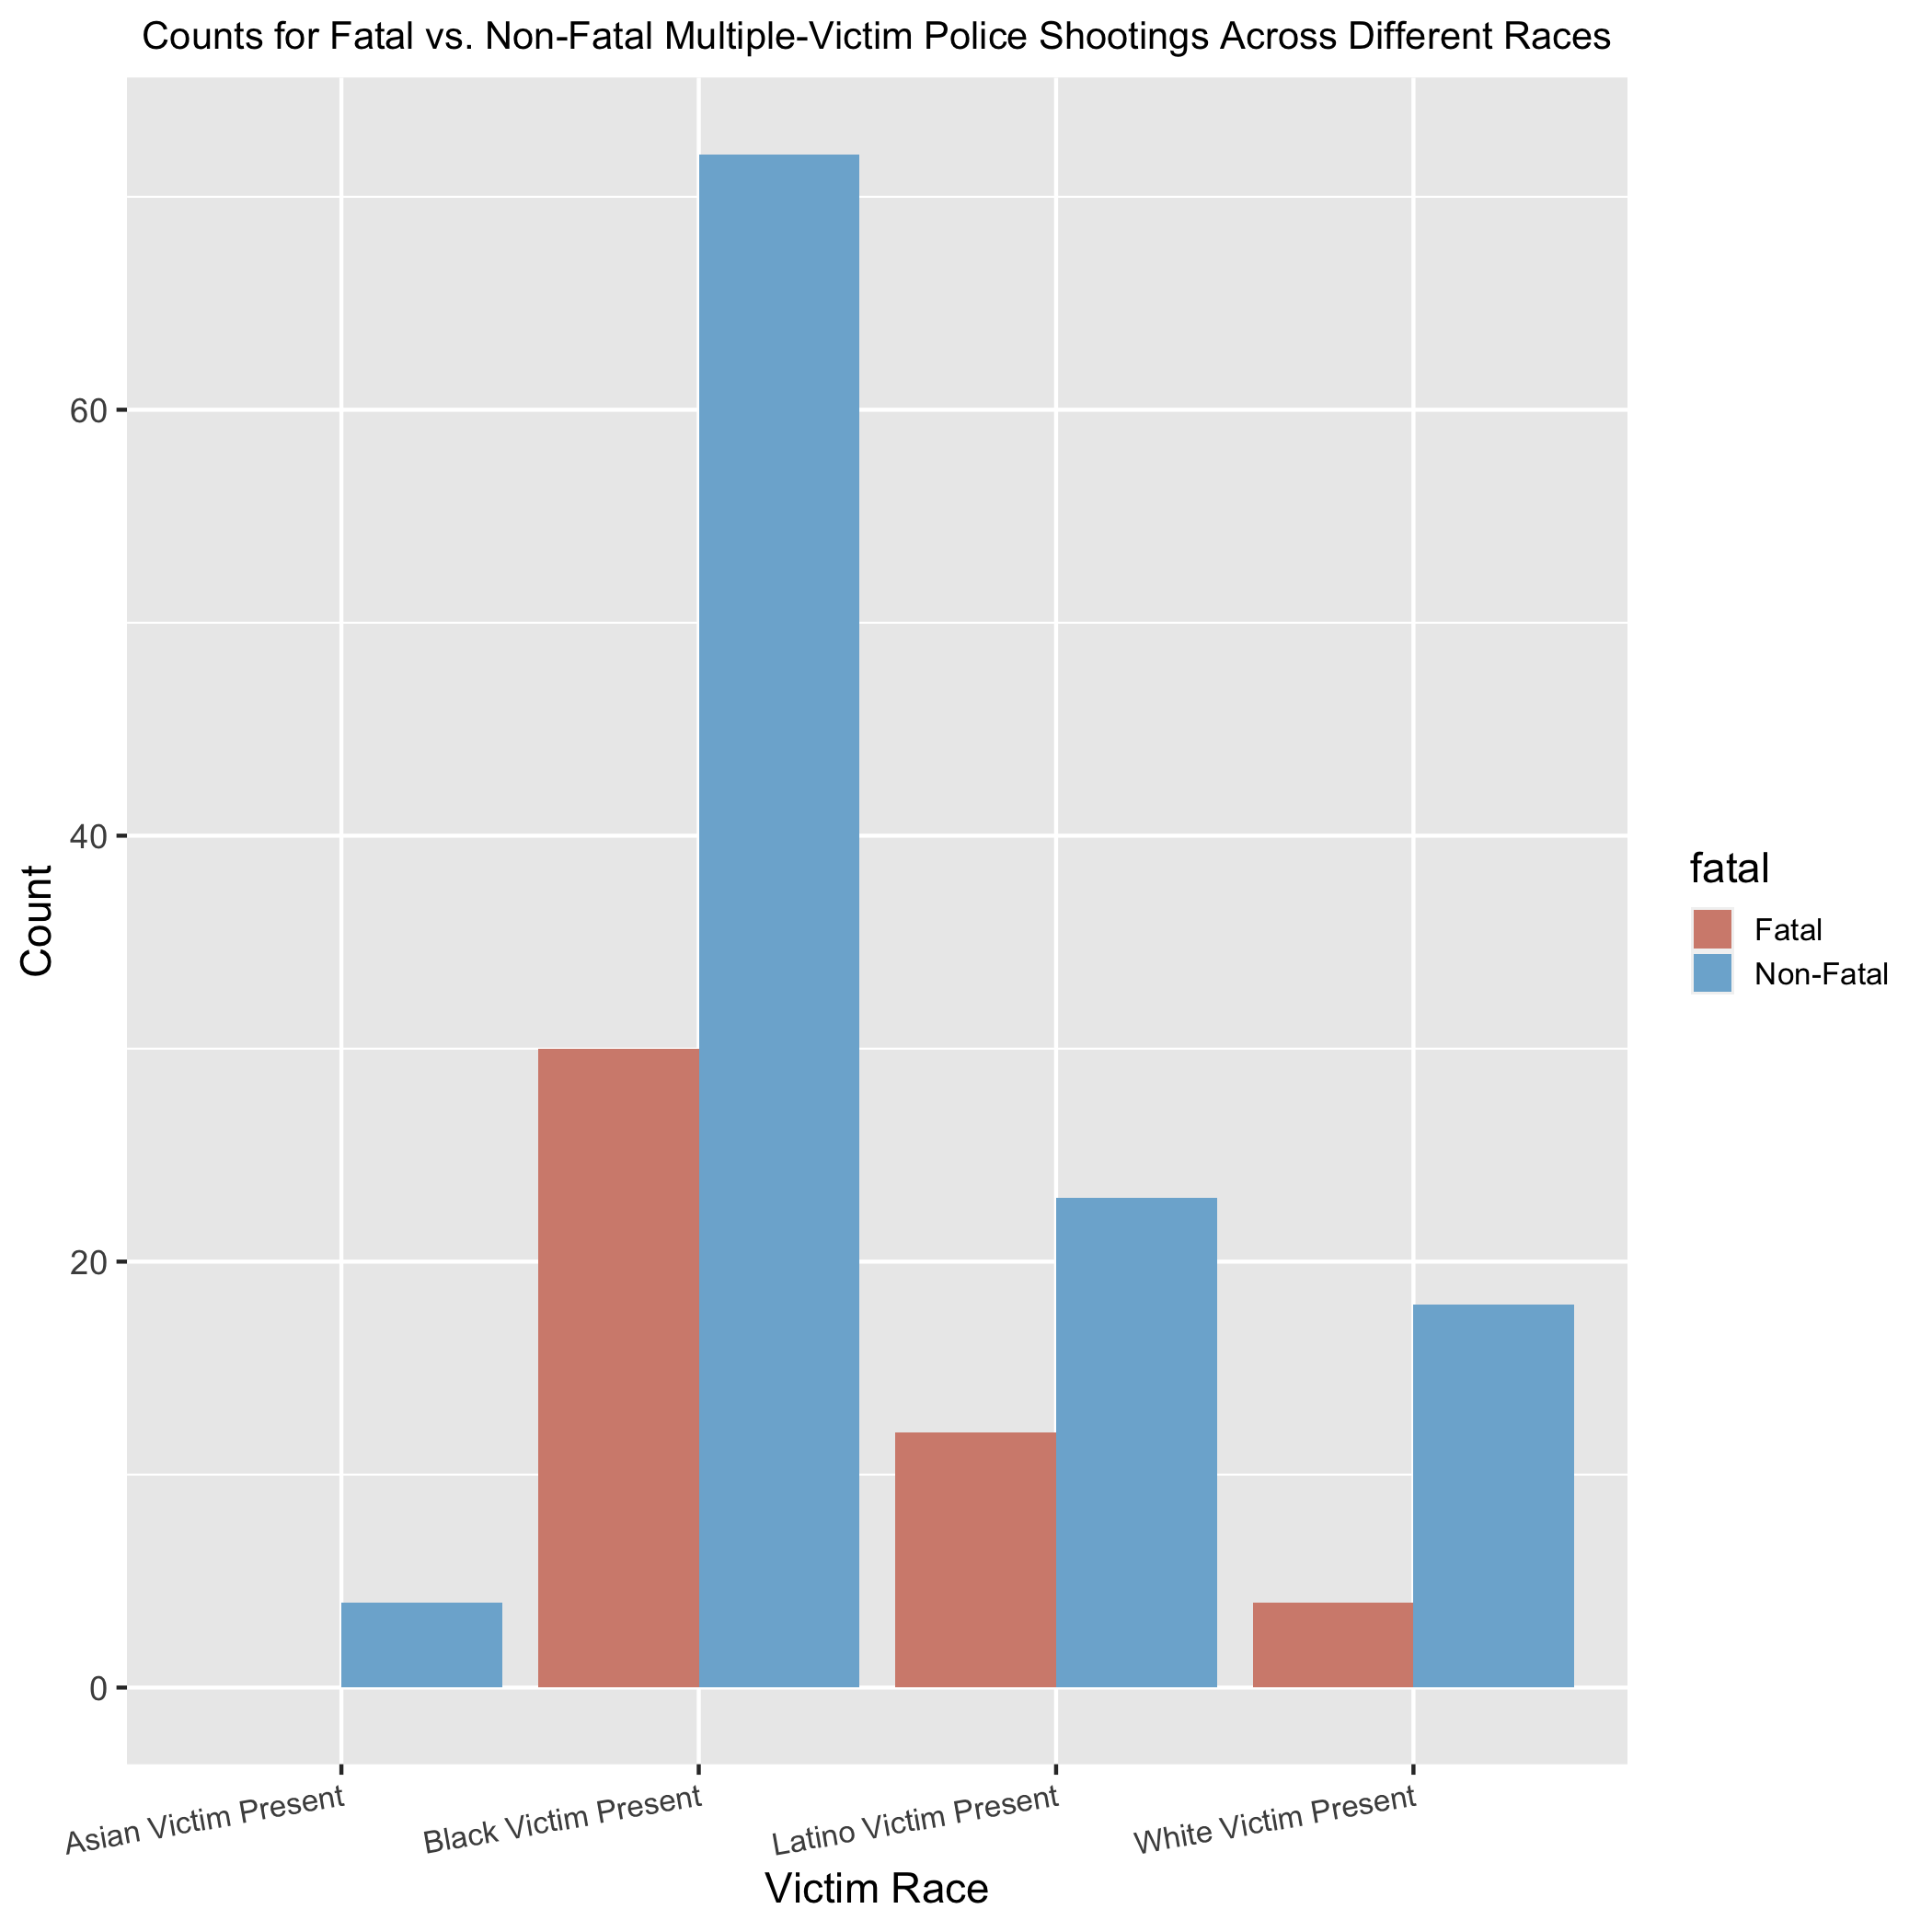
\includegraphics[width=0.5\linewidth]{figures/multeda1} 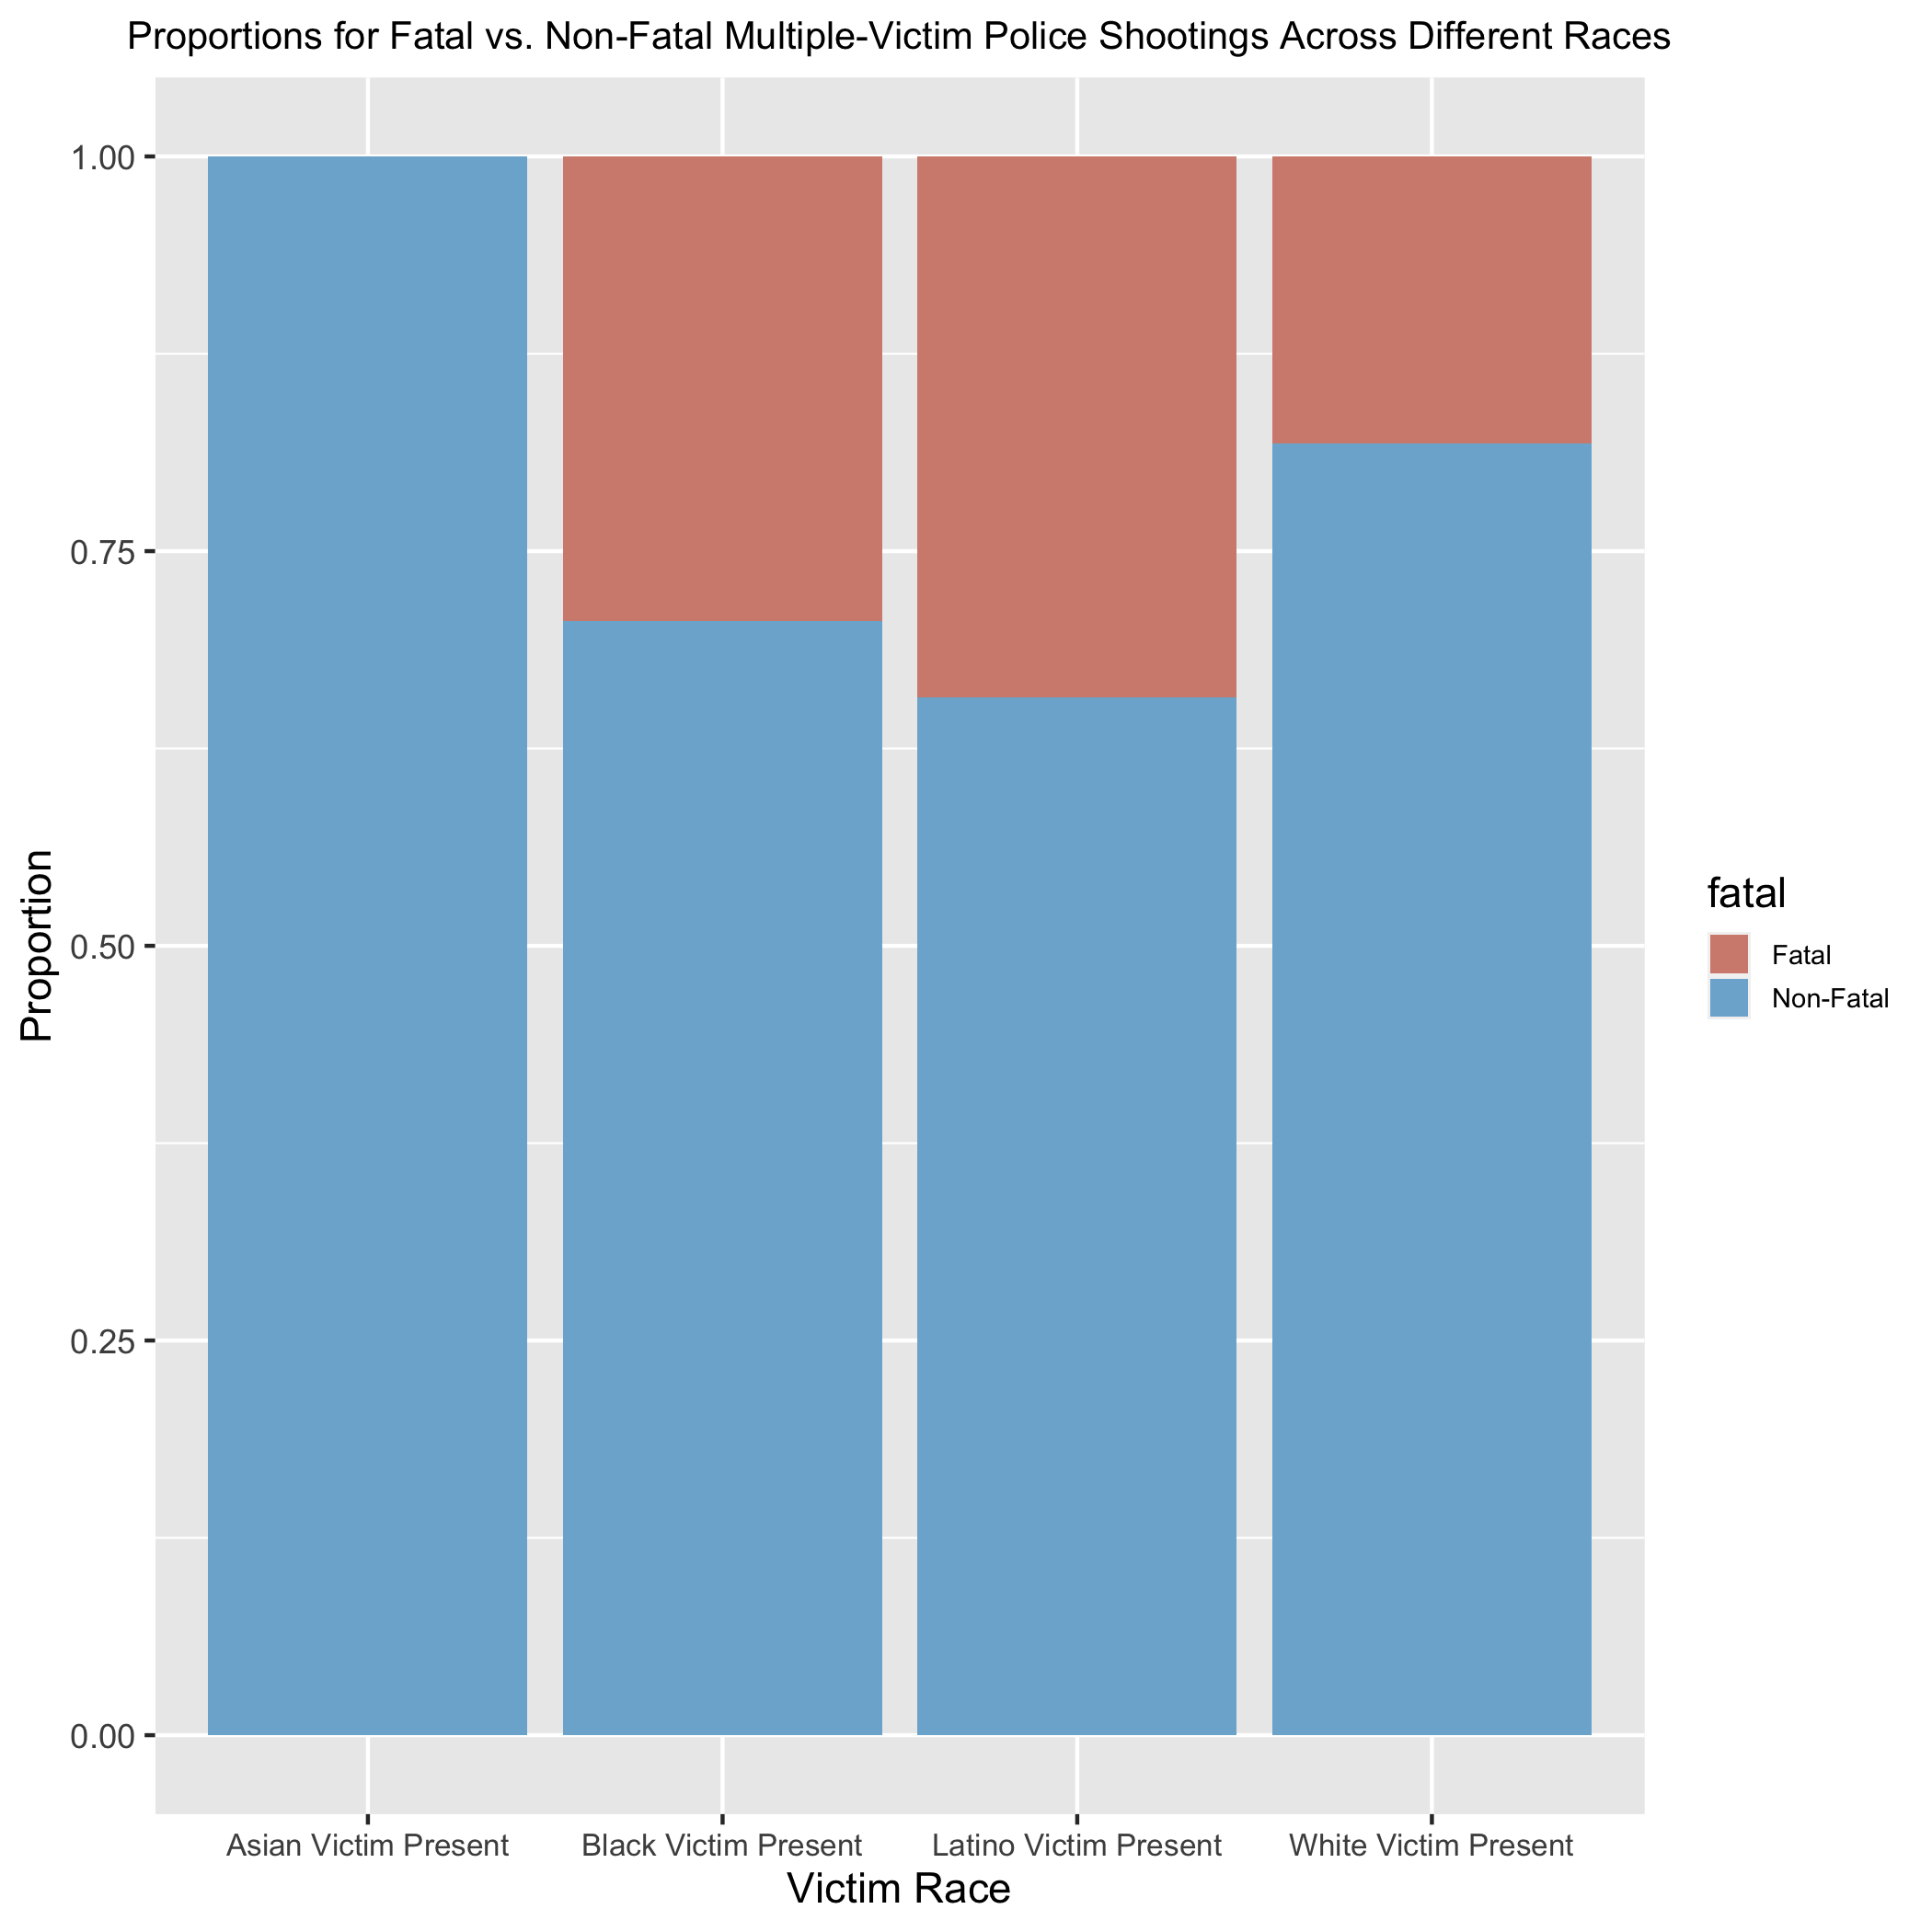
\includegraphics[width=0.5\linewidth]{figures/multeda2} \caption{Counts (left) and Proportions (right) of Different Races Across Multiple Victim Shootings}\label{fig:figures-mult}
\end{figure}

\begin{figure}
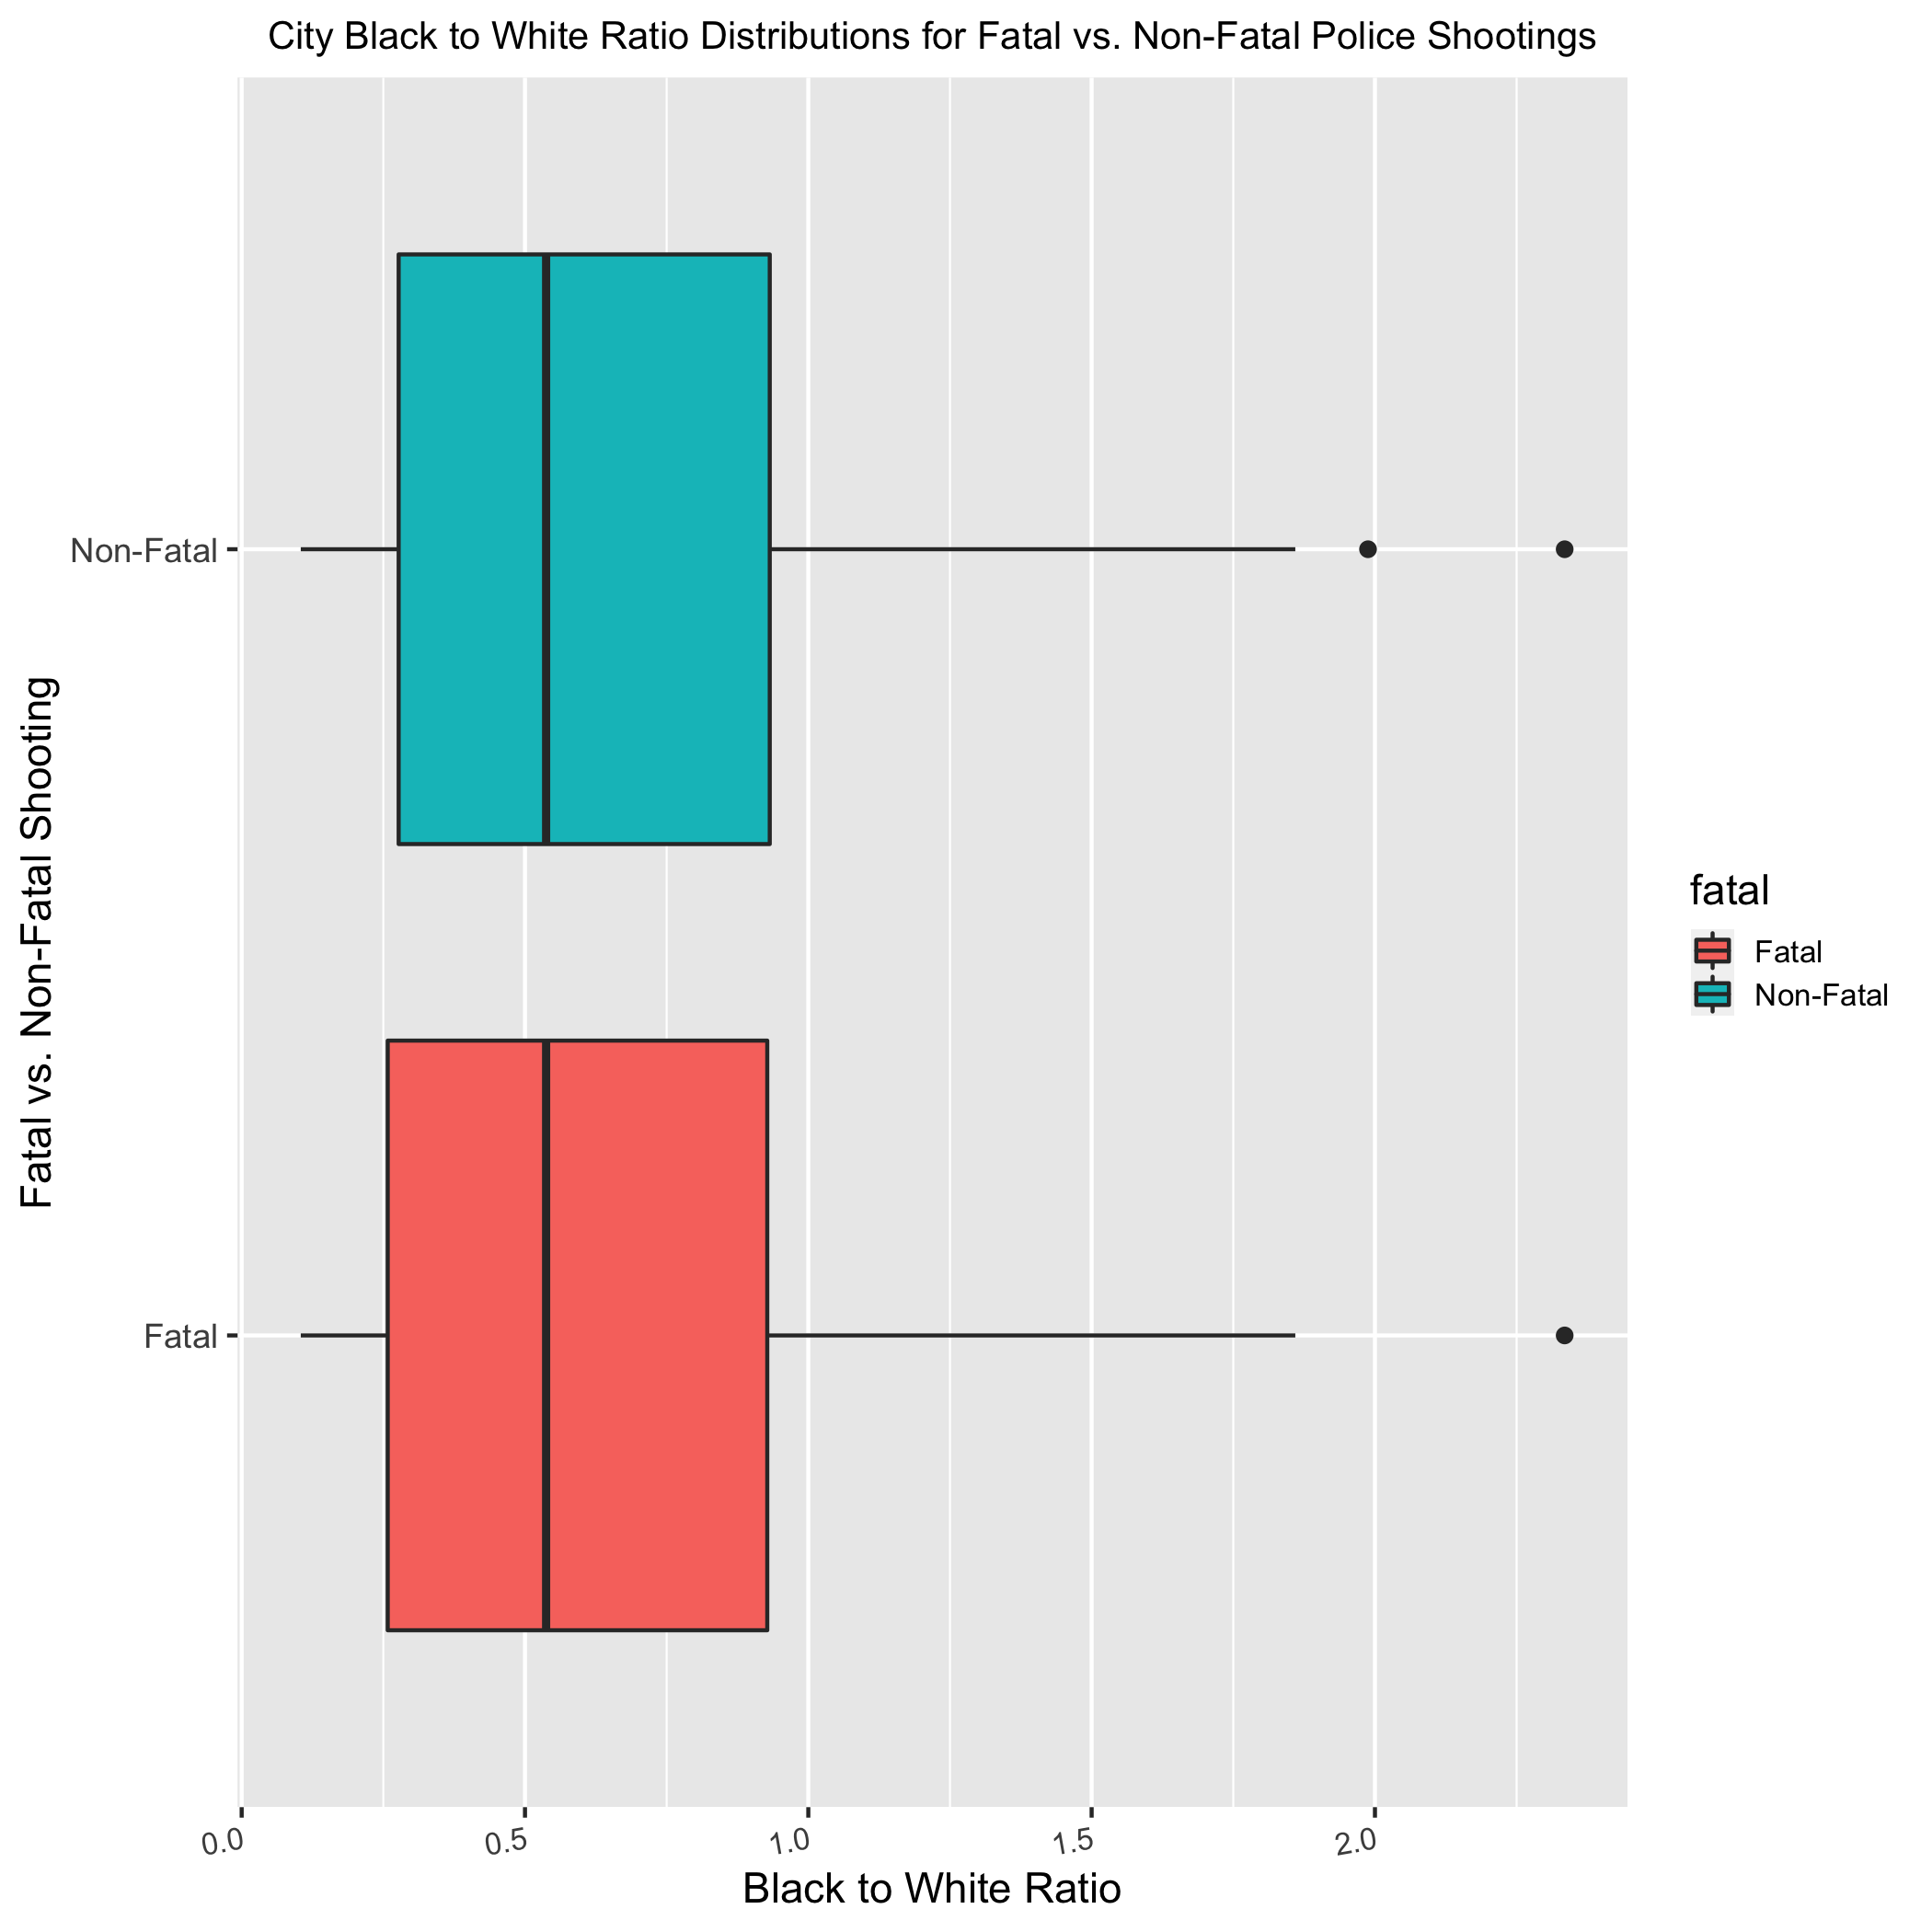
\includegraphics[width=0.5\linewidth]{figures/btweda} \caption{Proportion of Fatal Shootings vs. Black to White Ratios in Cities in Dataset}\label{fig:figures-btw}
\end{figure}

\begin{figure}
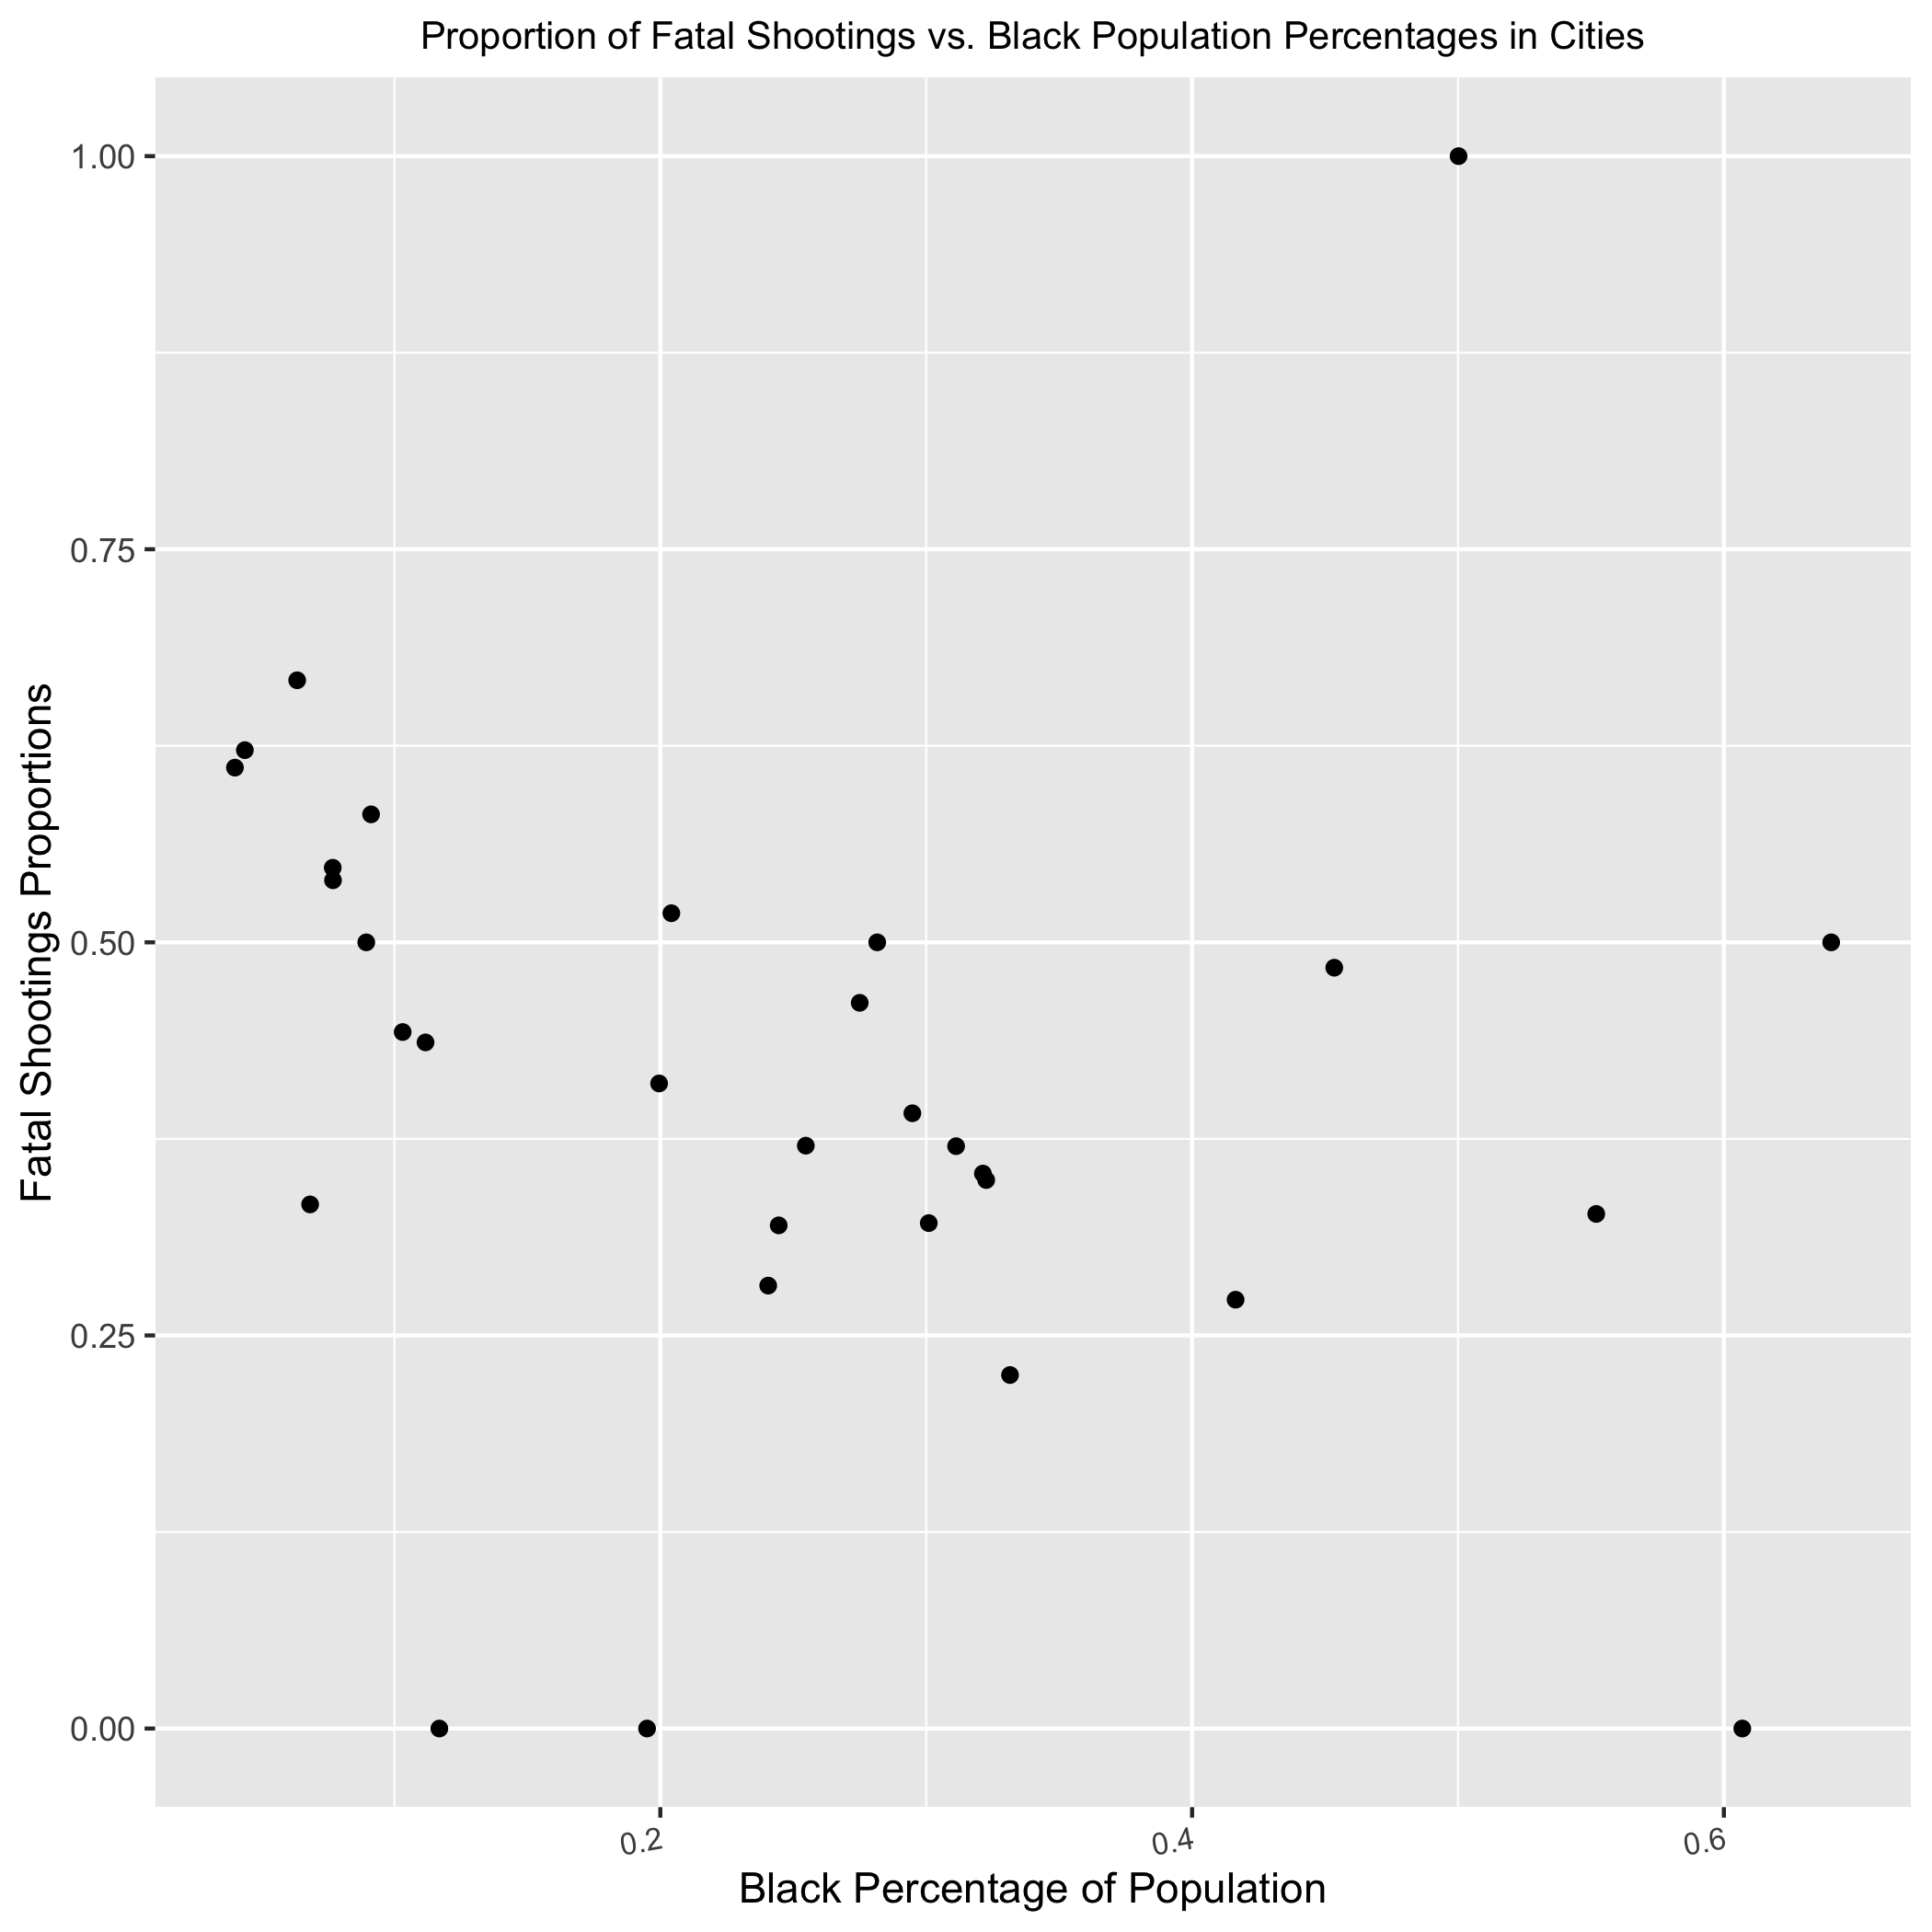
\includegraphics[width=0.5\linewidth]{figures/bpropeda} \caption{Proportion of Fatal Shootings vs. Black Population Percentages in Cities in Dataset}\label{fig:figures-bprop}
\end{figure}

\begin{figure}
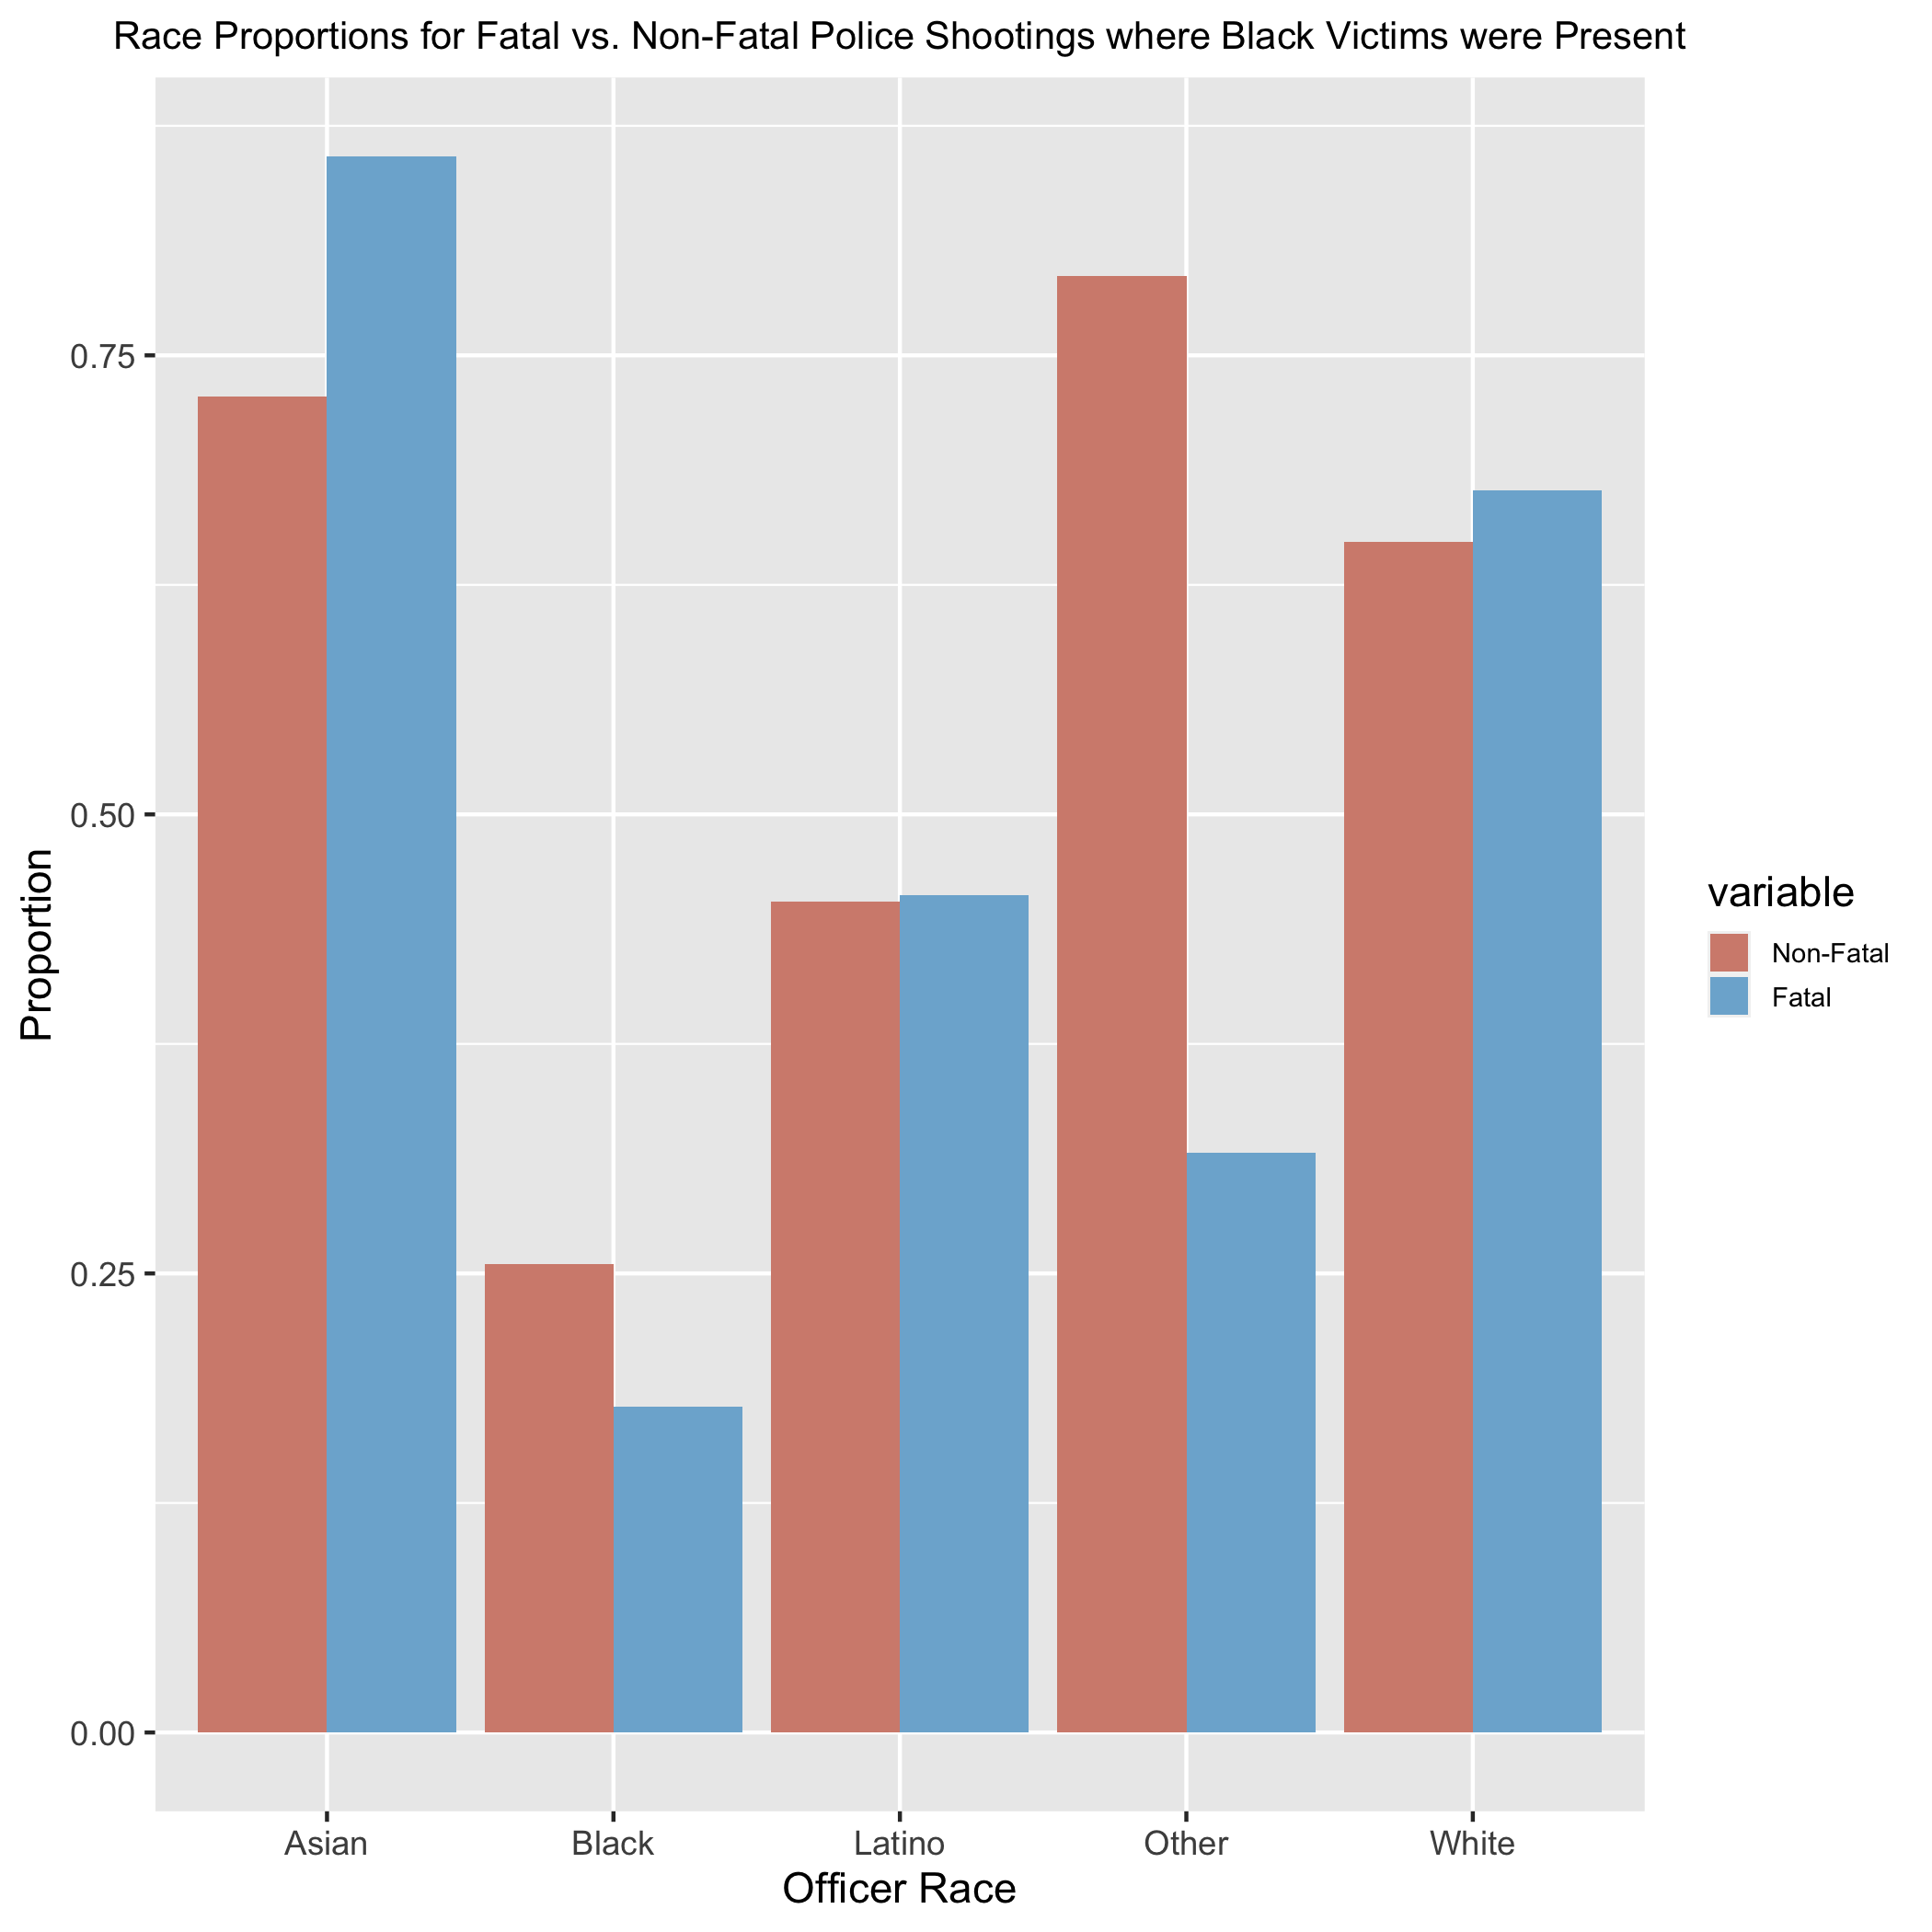
\includegraphics[width=0.5\linewidth]{figures/officerpropsb} \caption{Race Proportions for Fatal vs. Non-Fatal Police Shootings Where At Least One Black Victim was Present}\label{fig:figures-officersbprop}
\end{figure}

\end{document}
